%!TEX root = ../main.tex
\chapter{Dinamica dei sistemi di particelle}

\section{Sistemi di punti materiali}

Ci si sposta ora dalla dinamica del punto materiale alla dinamica dei sistemi di punti materiali. Essi sono sistemi in cui figurano numerosi oggetti ancora approssimati a corpi puntiformi che interagiscono tra di loro e contemporaneamente interagiscono con l'ambiente circostante.
Un approccio potrebbe essere quello di considerare ogni punto materiale e scrivere la seconda equazione della dinamica. Tuttavia si otterrebbe un sistema troppo complesso di questo tipo:

\[
	\begin{cases} \vec{F}_1^\text{tot}=m\vec{a}_1 \\ \vec{F}_2^\text{tot}=m\vec{a}_2 \\ \vdots \\ \vec{F}_n^\text{tot}=m\vec{a}_n  \end{cases} \text{ $n$ equazioni vettoriali in $3n$ incognite}
\]

In più non tutte le forze sono facilmente ricavabili a priori. I punti materiali ovviamente potranno scambiarsi delle forze, quindi ad esempio la massa $m_1$ interagendo con la massa $m_2$ sarà soggetta a una forza $F_1$. Inoltre, focalizzando l'attenzione sulla generica massa $i$-esima, questa non sarà solo soggetta all'interazione con gli altri corpi, ma anche a quella delle forze esterne, ad esempio la forza peso di attrazione al centro della Terra.

Si definiscono \textbf{forze esterne} le forze generate su un certo punto materiale sotto l'azione di parti esterne al sistema. Al contrario, le \textbf{forze interne} saranno quelle generate su una massa da un'altra parte del sistema.
La distinzione tra forze interne ed esterne dipende da come viene definito il sistema di punti. Se per esempio si ingloba nel sistema una parte del resto dell'universo, alcune forze, precedentemente considerate esterne, diventano interne.

Considerando la seconda legge della dinamica scritta per il corpo di massa $i$-esima, si può dire che la somma di tutte le forze che agiscono su di essa, danno luogo alla sua accelerazione vettoriale. Scomponendo tale somma nel contributo delle forze esterne e in quello delle forze interne:

\[
	\vec{F}_i^\text{ext}+\vec{F}_i^\text{int}=m\vec{a}_i
\]

Si è così definito dal punto di vista dinamico come cambia la terminologia quando si parla di dinamica dei sistemi.

È possibile anche parlare delle quantità di moto complessiva del sistema di punti. Si definisce \textbf{quantità di moto totale} di esso la somma vettoriale delle quantità di moto di ogni punto materiale.

\[
	\vec{p}_\text{tot}=\sum_{i=1}^n \vec{p}_i
\]

Si scrive la seconda legge della dinamica per tutti i punti fino all'$n$-esimo. Si troverà un sistema di $n$ equazioni vettoriali, cioè $3n$ equazioni scalari e quindi $3n$ incognite.

\[
	\begin{cases}
		\vec{F}_1^\text{int} + \vec{F}_1^\text{ext}=m\vec{a}_1=\frac{d\vec{p}_1}{dt} \\
		\vec{F}_2^\text{int} + \vec{F}_2^\text{ext}=m\vec{a}_2=\frac{d\vec{p}_2}{dt} \\
		\vdots \\
		\vec{F}_n^\text{int} + \vec{F}_n^\text{ext}=m\vec{a}_n=\frac{d\vec{p}_n}{dt}
	\end{cases}
\]

\paragraph{Esempio} Si consideri un portachiavi in cui ogni punto è una chiave. Quando lo si lancia, le varie chiavi sono soggette sicuramente all'azione della forza peso, ma esse in realtà non si muovono perché venendo a contatto con le chiavi vicine vengono spinte. Quindi l'azione delle forze interne va a modificare la traiettoria di ogni singolo punto. È impossibile riuscire a ricavare la loro azione per via dell'impossibilità di ricavare su di esse un'informazione quantitativa.

Quindi invece che risolvere il sistema in questa maniera, si va a generare un'unica equazione sommando membro a membro queste equazioni.

\[
	\sum_{i=1}^n \vec{F}_i^\text{ext}+\sum_{i=1}^n \vec{F}_i^\text{int}=\sum_{i=1}^nm_i\vec{a}_i=\frac{d\sum_{i=1}^n\vec{p}_i}{dt}=\frac{d\vec{p}_\text{tot}}{dt}
\]

La sommatoria delle forze interne si annulla perché per il principio di azione reazione per ogni forza interna ce ne sarà un'altra uguale e contraria. Si ottiene allora un'equazione in cui la sommatoria di tutte le forze esterne provocano la variazione della quantità di moto complessiva del sistema, eliminando le forze interne. La sommatoria delle forze esterne viene anche scritta come risultante delle forze esterne $\vec{R}_\text{tot}$:

\[
	\boxed{\vec{R}_\text{tot}=\frac{d\vec{p}_\text{tot}}{dt}}
\]

Questa equazione è un'equazione fondamentale che prende il nome di \textbf{prima equazione cardinale della dinamica dei sistemi}. Se si guarda un sistema di punti materiali ognuno dei quali si muove in maniera complicata, si può studiarne il moto complessivo in termini di quantità di moto, per poter così considerare soltanto l'effetto delle forze esterne. È una relazione molto comoda e sintetica da utilizzare.
Si dice che un sistema è \textbf{isolato} se la risultante delle forze esterne è uguale a zero. In questo caso la prima equazione diventa una legge di conservazione detta \textbf{principio di conservazione della quantità di moto}:

\[
	\boxed{\vec{R}^\text{est}=0 \implies \vec{p}_\text{tot}=\text{costante}}
\]

\paragraph{Esempio sulla legge di conservazione} Si immagini di avere un frammento (inizialmente fermo) sospeso in aria. Esso, a causa di una forza interna, esplode, rompendosi in due frammenti: il sistema è isolato.

\begin{figure}[htpb]
	\centering

	\tikzset{every picture/.style={line width=0.75pt}} %set default line width to 0.75pt        

	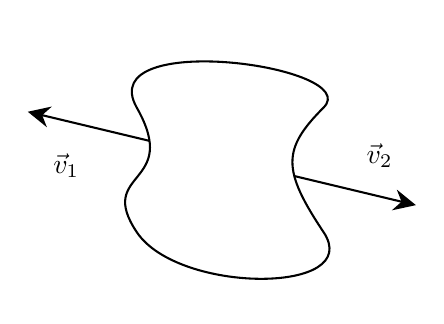
\begin{tikzpicture}[x=0.75pt,y=0.75pt,yscale=-1,xscale=1]
	%uncomment if require: \path (0,300); %set diagram left start at 0, and has height of 300

	%Shape: Polygon Curved [id:ds41536764033360196] 
	\draw   (134,95) .. controls (112.5,57) and (244,75) .. (224,95) .. controls (204,115) and (204,125) .. (224,155) .. controls (244,185) and (154,185) .. (134,155) .. controls (114,125) and (155.5,133) .. (134,95) -- cycle ;
	%Straight Lines [id:da7352415804326031] 
	\draw    (210,128) -- (265.58,141.3) ;
	\draw [shift={(268.5,142)}, rotate = 193.46] [fill={rgb, 255:red, 0; green, 0; blue, 0 }  ][line width=0.08]  [draw opacity=0] (10.72,-5.15) -- (0,0) -- (10.72,5.15) -- (7.12,0) -- cycle    ;
	%Straight Lines [id:da14490670515067294] 
	\draw    (84.42,97.7) -- (140,111) ;
	\draw [shift={(81.5,97)}, rotate = 13.46] [fill={rgb, 255:red, 0; green, 0; blue, 0 }  ][line width=0.08]  [draw opacity=0] (10.72,-5.15) -- (0,0) -- (10.72,5.15) -- (7.12,0) -- cycle    ;

	% Text Node
	\draw (100,123) node    {$\vec{v}_{1}$};
	% Text Node
	\draw (251,118) node    {$\vec{v}_{2}$};

	\end{tikzpicture}
\end{figure}
\FloatBarrier
Se uno di essi si muove in una direzione, l'altro frammento partirà in direzione uguale e contraria. Questo perché il sistema era inizialmente fermo e quindi, la quantità di moto che era zero inizialmente, deve continuare a essere tale. Il sistema rimane complessivamente fermo anche se in realtà i frammenti partono in direzione opposta. Essi non hanno necessariamente la stessa velocità, perché quello che si deve osservare è la quantità di moto totale, cioè la somma:

\[
	m_1\vec{v}_1+m_2\vec{v}_2=0
\]
È evidente che il frammento di massa maggiore partirà con una velocità minore in modulo.

\section{Centro di massa}

Si immagini di avere $n$ punti materiali, rilevati rispetto a un osservatore assoluto. È possibile definire la posizione di un punto fittizio detto \textbf{centro di massa}, il cui vettore posizione è dato dalla posizione media di tutti i punti materiali pesati per la loro massa. Attuare una media ponderata di questo tipo significa dare più importanza alle masse più elevate. Il centro di massa di un sistema tende a trovarsi dove è concentrata maggiormente la sua massa e non coincide necessariamente con un suo punto. La definizione matematica è:

\[
	\boxed{\vec{r}_\text{CM} =\sum_{i=1}^n \frac{m_i\vec{r}_i}{M_\text{tot}}}
\]

\begin{figure}[htpb]
	\centering

	\tikzset{every picture/.style={line width=0.75pt}} %set default line width to 0.75pt        

	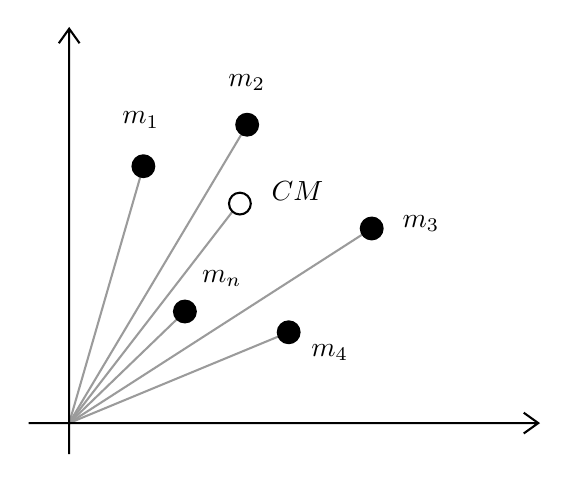
\begin{tikzpicture}[x=0.75pt,y=0.75pt,yscale=-1,xscale=1]
	%uncomment if require: \path (0,300); %set diagram left start at 0, and has height of 300

	%Straight Lines [id:da9212332807493775] 
	\draw [color={rgb, 255:red, 155; green, 155; blue, 155 }  ,draw opacity=1 ]   (105.25,118.25) -- (69.5,242) ;
	%Straight Lines [id:da44266553778346474] 
	\draw [color={rgb, 255:red, 155; green, 155; blue, 155 }  ,draw opacity=1 ]   (155.25,98.25) -- (69.5,242) ;
	%Straight Lines [id:da29671944764078395] 
	\draw [color={rgb, 255:red, 155; green, 155; blue, 155 }  ,draw opacity=1 ]   (215.25,148.25) -- (69.5,242) ;
	%Straight Lines [id:da9922801504038579] 
	\draw [color={rgb, 255:red, 155; green, 155; blue, 155 }  ,draw opacity=1 ]   (175.25,198.25) -- (69.5,242) ;
	%Straight Lines [id:da04217664681854427] 
	\draw [color={rgb, 255:red, 155; green, 155; blue, 155 }  ,draw opacity=1 ]   (125.25,188.25) -- (69.5,242) ;
	%Straight Lines [id:da7222564679512768] 
	\draw [color={rgb, 255:red, 155; green, 155; blue, 155 }  ,draw opacity=1 ]   (148.4,139.8) -- (69.5,242) ;
	%Shape: Axis 2D [id:dp29791761046641163] 
	\draw  (50,242) -- (295.5,242)(69.5,52) -- (69.5,257) (288.5,237) -- (295.5,242) -- (288.5,247) (64.5,59) -- (69.5,52) -- (74.5,59)  ;
	%Shape: Circle [id:dp7005511906572408] 
	\draw  [fill={rgb, 255:red, 0; green, 0; blue, 0 }  ,fill opacity=1 ] (100,118.25) .. controls (100,115.35) and (102.35,113) .. (105.25,113) .. controls (108.15,113) and (110.5,115.35) .. (110.5,118.25) .. controls (110.5,121.15) and (108.15,123.5) .. (105.25,123.5) .. controls (102.35,123.5) and (100,121.15) .. (100,118.25) -- cycle ;
	%Shape: Circle [id:dp36061172179055134] 
	\draw  [fill={rgb, 255:red, 0; green, 0; blue, 0 }  ,fill opacity=1 ] (150,98.25) .. controls (150,95.35) and (152.35,93) .. (155.25,93) .. controls (158.15,93) and (160.5,95.35) .. (160.5,98.25) .. controls (160.5,101.15) and (158.15,103.5) .. (155.25,103.5) .. controls (152.35,103.5) and (150,101.15) .. (150,98.25) -- cycle ;
	%Shape: Circle [id:dp6157944650911422] 
	\draw  [fill={rgb, 255:red, 0; green, 0; blue, 0 }  ,fill opacity=1 ] (170,198.25) .. controls (170,195.35) and (172.35,193) .. (175.25,193) .. controls (178.15,193) and (180.5,195.35) .. (180.5,198.25) .. controls (180.5,201.15) and (178.15,203.5) .. (175.25,203.5) .. controls (172.35,203.5) and (170,201.15) .. (170,198.25) -- cycle ;
	%Shape: Circle [id:dp9455255125788649] 
	\draw  [fill={rgb, 255:red, 0; green, 0; blue, 0 }  ,fill opacity=1 ] (210,148.25) .. controls (210,145.35) and (212.35,143) .. (215.25,143) .. controls (218.15,143) and (220.5,145.35) .. (220.5,148.25) .. controls (220.5,151.15) and (218.15,153.5) .. (215.25,153.5) .. controls (212.35,153.5) and (210,151.15) .. (210,148.25) -- cycle ;
	%Shape: Circle [id:dp7342008389787866] 
	\draw  [fill={rgb, 255:red, 0; green, 0; blue, 0 }  ,fill opacity=1 ] (120,188.25) .. controls (120,185.35) and (122.35,183) .. (125.25,183) .. controls (128.15,183) and (130.5,185.35) .. (130.5,188.25) .. controls (130.5,191.15) and (128.15,193.5) .. (125.25,193.5) .. controls (122.35,193.5) and (120,191.15) .. (120,188.25) -- cycle ;
	%Shape: Circle [id:dp8542177920959095] 
	\draw   (146.5,136.25) .. controls (146.5,133.35) and (148.85,131) .. (151.75,131) .. controls (154.65,131) and (157,133.35) .. (157,136.25) .. controls (157,139.15) and (154.65,141.5) .. (151.75,141.5) .. controls (148.85,141.5) and (146.5,139.15) .. (146.5,136.25) -- cycle ;

	% Text Node
	\draw (104,96) node    {$m_{1}$};
	% Text Node
	\draw (155,78) node    {$m_{2}$};
	% Text Node
	\draw (239,146) node    {$m_{3}$};
	% Text Node
	\draw (195,208) node    {$m_{4}$};
	% Text Node
	\draw (143,172.5) node    {$m_{n}$};
	% Text Node
	\draw (179.5,130) node    {$CM$};

	\end{tikzpicture}
\end{figure}
\FloatBarrier
Definita la posizione del centro di massa, si può anche definire la sua velocità, derivando la relazione:

\[
	\vec{v}_\text{CM}=\frac{d\vec{r}_\text{CM}}{dt}=\frac{d\sum_{i=1}^nm_i\vec{r}_i}{dt} \frac{1}{M_\text{tot}}=\sum_{i=1}^n\frac{dm_i\vec{r}_i}{dt} \frac{1}{M_\text{tot}}=\frac{\sum_{i=1}^nm_i\vec{v}_i}{M_\text{tot}}
\]

La velocità del centro di massa non è altro che la media delle velocità dei punti materiali pesata per le corrispondenti masse. Da questo risultato si ottiene un'informazione molto importante sul centro di massa. Infatti:

\[
	\boxed{M_\text{tot}\vec{v}_\text{CM}=\sum_{i=1}^nm_i \vec{v}_i=\vec{p}_\text{tot}}
\]

Questo risultato prende il nome di \textbf{primo teorema del centro di massa}. In termini di quantità di moto, si può considerare il sistema nel suo complesso come un unico punto materiale in cui è concentrata tutta la massa e che coincide con la posizione del centro di massa. Si va ad applicare questo risultato alla prima equazione cardinale della dinamica. Nell'ipotesi che il sistema non vari la sua massa:

\[
	\boxed{\vec{R}_\text{tot}=\frac{d\vec{p}_\text{tot}}{dt}=\frac{dM_\text{tot}\vec{v}_\text{CM}}{dt}=M_\text{tot}\frac{d\vec{v}_\text{CM}}{dt}=M_\text{tot}\vec{a}_\text{CM}}
\]

L'accelerazione del centro di massa è la media pesata delle varie accelerazioni. Si vede quindi che il suo moto è causato dalle forze esterne.  Questo risultato prende il nome di \textbf{secondo teorema del centro di massa} e, dal punto di vista delle informazioni che fornisce, è del tutto equivalente alla prima equazione cardinale della dinamica. Il suo vantaggio è che fa vedere il problema dello studio del sistema di punti materiali in maniera molto semplice.
In aggiunta esso può diventare un principio di conservazione quando sul sistema non agiscono forze esterne. In questo caso il centro di massa si muove di moto rettilineo uniforme o, se era inizialmente fermo, rimane in quiete.
Si è ridotto il complesso problema dello studio del moto di un sistema di punti materiali allo studio del moto di un singolo punto materiale che è il centro di massa.

\paragraph{Esempio} Se il sistema è isolato, le equazioni ottenute diventano:

\[
	\vec{R}_\text{ext}=0 \quad \vec{a}_\text{CM}=0 \quad \vec{v}_\text{CM}=\text{cost}
\]

Il centro di massa si muove di moto rettilineo uniforme, di cui la quiete è un caso particolare. Questa relazione è interessante anche quando il sistema non è isolato nel suo complesso ma in una sola direzione. Per capire ciò, si immagini di avere un cannone di massa $M$, con dentro una massa $m$. Inizialmente il sistema è fermo, ad un certo istante il cannone viene innescato e la palla parte con una certa velocità nota $\vec{v}_0$.

\begin{figure}[htpb]
	\centering

	\tikzset{every picture/.style={line width=0.75pt}} %set default line width to 0.75pt        

	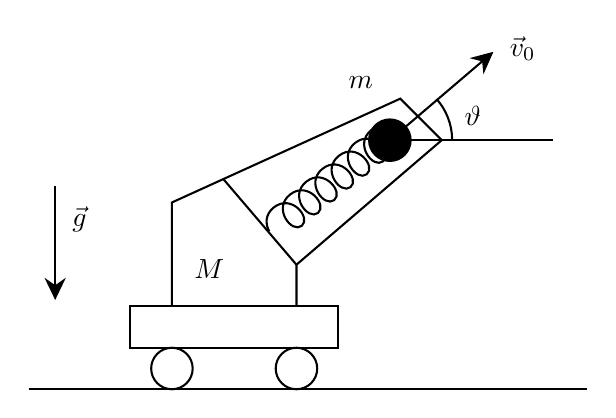
\begin{tikzpicture}[x=0.75pt,y=0.75pt,yscale=-1,xscale=1]
	%uncomment if require: \path (0,300); %set diagram left start at 0, and has height of 300

	%Straight Lines [id:da8804303858640294] 
	\draw    (61,210) -- (330,210) ;
	%Shape: Circle [id:dp6243569737365466] 
	\draw   (120,200) .. controls (120,194.48) and (124.48,190) .. (130,190) .. controls (135.52,190) and (140,194.48) .. (140,200) .. controls (140,205.52) and (135.52,210) .. (130,210) .. controls (124.48,210) and (120,205.52) .. (120,200) -- cycle ;
	%Shape: Circle [id:dp5679046904606062] 
	\draw   (180,200) .. controls (180,194.48) and (184.48,190) .. (190,190) .. controls (195.52,190) and (200,194.48) .. (200,200) .. controls (200,205.52) and (195.52,210) .. (190,210) .. controls (184.48,210) and (180,205.52) .. (180,200) -- cycle ;
	%Shape: Rectangle [id:dp6403059717351121] 
	\draw   (110,170) -- (210,170) -- (210,190) -- (110,190) -- cycle ;
	%Straight Lines [id:da5020169261481033] 
	\draw    (130,170) -- (130,120) -- (240,70) -- (260,90) -- (190,150) -- (190,170) ;
	%Straight Lines [id:da3957252727046501] 
	\draw    (155,109) -- (190,150) ;
	%Shape: Circle [id:dp32993320697849726] 
	\draw  [fill={rgb, 255:red, 0; green, 0; blue, 0 }  ,fill opacity=1 ] (225,90) .. controls (225,84.48) and (229.48,80) .. (235,80) .. controls (240.52,80) and (245,84.48) .. (245,90) .. controls (245,95.52) and (240.52,100) .. (235,100) .. controls (229.48,100) and (225,95.52) .. (225,90) -- cycle ;
	%Shape: Spring [id:dp6487389658408163] 
	\draw   (176.89,133.92) .. controls (175,130.53) and (174.77,125.82) .. (179.08,122.4) .. controls (187.7,115.56) and (197.22,127.56) .. (192.52,131.29) .. controls (187.82,135.02) and (178.3,123.02) .. (186.91,116.19) .. controls (195.53,109.35) and (205.05,121.35) .. (200.35,125.08) .. controls (195.65,128.81) and (186.13,116.81) .. (194.75,109.97) .. controls (203.36,103.13) and (212.88,115.13) .. (208.18,118.86) .. controls (203.48,122.59) and (193.96,110.59) .. (202.58,103.75) .. controls (211.2,96.92) and (220.72,108.92) .. (216.02,112.65) .. controls (211.32,116.38) and (201.8,104.38) .. (210.41,97.54) .. controls (219.03,90.7) and (228.55,102.7) .. (223.85,106.43) .. controls (219.15,110.16) and (209.63,98.16) .. (218.25,91.32) .. controls (226.86,84.49) and (236.39,96.49) .. (231.69,100.22) .. controls (226.99,103.95) and (217.46,91.95) .. (226.08,85.11) .. controls (227.27,84.16) and (228.48,83.58) .. (229.67,83.28) ;
	%Shape: Boxed Line [id:dp10601723496206072] 
	\draw    (235,90) -- (282.59,49.37) ;
	\draw [shift={(284.88,47.42)}, rotate = 499.51] [fill={rgb, 255:red, 0; green, 0; blue, 0 }  ][line width=0.08]  [draw opacity=0] (10.72,-5.15) -- (0,0) -- (10.72,5.15) -- (7.12,0) -- cycle    ;
	%Straight Lines [id:da13288739314820308] 
	\draw    (235,90) -- (313.75,90) ;
	%Straight Lines [id:da24008536549031012] 
	\draw    (73.75,164) -- (73.75,112) ;
	\draw [shift={(73.75,167)}, rotate = 270] [fill={rgb, 255:red, 0; green, 0; blue, 0 }  ][line width=0.08]  [draw opacity=0] (10.72,-5.15) -- (0,0) -- (10.72,5.15) -- (7.12,0) -- cycle    ;
	%Shape: Arc [id:dp08315862136385044] 
	\draw  [draw opacity=0] (257.48,70.13) .. controls (262.06,75.31) and (264.88,82.08) .. (265,89.5) -- (235,90) -- cycle ; \draw   (257.48,70.13) .. controls (262.06,75.31) and (264.88,82.08) .. (265,89.5) ;

	% Text Node
	\draw (85.5,128) node    {$\vec{g}$};
	% Text Node
	\draw (299,46) node    {$\vec{v}_{0}$};
	% Text Node
	\draw (221,62) node    {$m$};
	% Text Node
	\draw (275,78.25) node    {$\vartheta $};
	% Text Node
	\draw (148,152) node    {$M$};

	\end{tikzpicture}
\end{figure}
\FloatBarrier
Si sa che il piano su cui è appoggiato il cannone è perfettamente liscio. Quando si spara la palla il cannone rincula indietro. Il sistema infatti non è isolato ma vi è la forza peso, per cui agisce una forza esterna in direzione verticale. In direzione parallela al piano però non c'è alcuna forza esterna. Questo vuole dire che allora il sistema è isolato in una certa direzione, in questo caso la $x$. Allora si conserva la componente lungo essa della velocità del centro di massa. La sua velocità inizialmente era zero. Quando il cannone spara, per il principio di azione e reazione, il cannone viene spinto indietro. Se la velocità iniziale è zero, lo sarà anche quando la palla di cannone è partita.

\[
	\frac{mv_0 \cos\vartheta+ Mv*}{m+M} =0
\]

Si ottiene:

\[
	v*=-\frac{m}{M}v_0\cos\vartheta
\]

Il cannone va indietro con una velocità molto piccola a causa della sua massa elevata.

\[
	\norm{\vec{v}_c}=\frac{mv_0\cos\vartheta}{M}
\]

In direzione $y$, le forze, entrambe esterne, sono la reazione normale e la forza peso. La responsabile dell'impulso è la reazione normale. Essa inizialmente serve solo a bilanciare il peso della palla di cannone, ma nel momento in cui la palla viene sparata, riceve una variazione molto intesa del suo valore, che quindi aumenta istantaneamente.

La variazione di quantità di moto in direzione $y$ sarà:

\[
	\Delta p_{\text{tot},y}=mv_0\sin\vartheta-0
\]

Questo effetto lo da l'impulso della reazione normale nell'intervallo di tempo $\Delta t$ dello sparo. Si può calcolare il valore medio della reazione normale:

\[
	\Delta p_{\text{tot},y}=mv_0\sin\vartheta=\int_0^{\Delta t} R_n \,dt=\bar{R}_n\Delta t
\]

Si ha ora un corpo rigido, somma di tanti punti materiali. Questo può ruotare in molti modi intorno al suo centro di massa senza che esso si sposti. In tal caso il teorema sul centro di massa non dice nulla. Bisogna aggiungere ancora qualche informazione per capire come descrivere complessivamente il moto di un sistema di questo tipo.
Per capire come un corpo ruota attorno a un centro di massa, si deve richiamare il teorema del momento angolare, il quale afferma che se un punto materiale è soggetto a una risultante delle forze che genera un momento rispetto ad un certo polo $O$, l'azione dinamica a cui dà luogo il moto delle forze, è quello di far variare nel tempo il momento angolare di esso.

\begin{figure}[htpb]
	\centering

	\tikzset{every picture/.style={line width=0.75pt}} %set default line width to 0.75pt        

	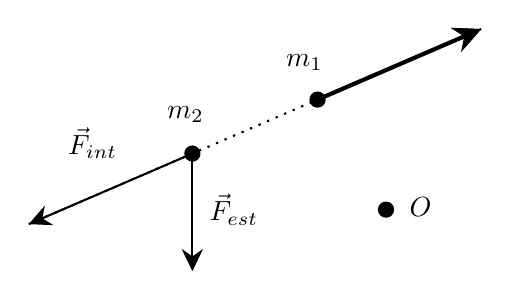
\begin{tikzpicture}[x=0.75pt,y=0.75pt,yscale=-1,xscale=1]
	%uncomment if require: \path (0,300); %set diagram left start at 0, and has height of 300

	%Straight Lines [id:da9001806911610699] 
	\draw  [dash pattern={on 0.84pt off 2.51pt}]  (98.5,185) -- (316.5,91) ;
	%Straight Lines [id:da13465404967438555] 
	\draw [line width=0.75]    (101.25,183.81) -- (177.35,151) ;
	\draw [shift={(98.5,185)}, rotate = 336.67] [fill={rgb, 255:red, 0; green, 0; blue, 0 }  ][line width=0.08]  [draw opacity=0] (10.72,-5.15) -- (0,0) -- (10.72,5.15) -- (7.12,0) -- cycle    ;
	%Straight Lines [id:da13465404967438555] 
	\draw [line width=1.5]    (237.65,125) -- (312.83,92.58) ;
	\draw [shift={(316.5,91)}, rotate = 516.6700000000001] [fill={rgb, 255:red, 0; green, 0; blue, 0 }  ][line width=0.08]  [draw opacity=0] (13.4,-6.43) -- (0,0) -- (13.4,6.44) -- (8.9,0) -- cycle    ;
	%Straight Lines [id:da3937309759048766] 
	\draw [line width=0.75]    (237.65,125) -- (313.75,92.19) ;
	\draw [shift={(316.5,91)}, rotate = 516.6700000000001] [fill={rgb, 255:red, 0; green, 0; blue, 0 }  ][line width=0.08]  [draw opacity=0] (10.72,-5.15) -- (0,0) -- (10.72,5.15) -- (7.12,0) -- cycle    ;
	%Shape: Circle [id:dp12362703310493028] 
	\draw  [fill={rgb, 255:red, 0; green, 0; blue, 0 }  ,fill opacity=1 ] (173.95,151) .. controls (173.95,149.12) and (175.47,147.6) .. (177.35,147.6) .. controls (179.23,147.6) and (180.75,149.12) .. (180.75,151) .. controls (180.75,152.88) and (179.23,154.4) .. (177.35,154.4) .. controls (175.47,154.4) and (173.95,152.88) .. (173.95,151) -- cycle ;
	%Shape: Circle [id:dp3472803664189661] 
	\draw  [fill={rgb, 255:red, 0; green, 0; blue, 0 }  ,fill opacity=1 ] (234.25,125) .. controls (234.25,123.12) and (235.77,121.6) .. (237.65,121.6) .. controls (239.53,121.6) and (241.05,123.12) .. (241.05,125) .. controls (241.05,126.88) and (239.53,128.4) .. (237.65,128.4) .. controls (235.77,128.4) and (234.25,126.88) .. (234.25,125) -- cycle ;
	%Shape: Circle [id:dp32662397763234785] 
	\draw  [fill={rgb, 255:red, 0; green, 0; blue, 0 }  ,fill opacity=1 ] (267.25,178) .. controls (267.25,176.12) and (268.77,174.6) .. (270.65,174.6) .. controls (272.53,174.6) and (274.05,176.12) .. (274.05,178) .. controls (274.05,179.88) and (272.53,181.4) .. (270.65,181.4) .. controls (268.77,181.4) and (267.25,179.88) .. (267.25,178) -- cycle ;
	%Straight Lines [id:da43912600871808216] 
	\draw [line width=0.75]    (177.35,204.67) -- (177.35,151) ;
	\draw [shift={(177.35,207.67)}, rotate = 270] [fill={rgb, 255:red, 0; green, 0; blue, 0 }  ][line width=0.08]  [draw opacity=0] (10.72,-5.15) -- (0,0) -- (10.72,5.15) -- (7.12,0) -- cycle    ;

	% Text Node
	\draw (129.33,146) node    {$\vec{F}_{int}$};
	% Text Node
	\draw (197.33,178) node    {$\vec{F}_{est}$};
	% Text Node
	\draw (174,132) node    {$m_{2}$};
	% Text Node
	\draw (231.33,107.33) node    {$m_{1}$};
	% Text Node
	\draw (287.33,176.67) node    {$O$};

	\end{tikzpicture}
\end{figure}
\FloatBarrier
Si applica tale teorema a un sistema di punti materiali. Si mette in evidenza per ognuna delle masse un certo polo $O$ e si calcola per ogni forza il momento generato. Le forze si distinguono sempre in interne ed esterne.

\[
	\vec{M}_1^{\text{int}, (o)}+\vec{M}_1^{\text{ext}, (o)}=\frac{d\vec{L_1}}{dt}+\vec{v}_0\times m_1\vec{v}_1
\]

Si va a riscrivere la relazione tutte le masse fino alla massa $n$-esima.

\[
	\vec{M}_n^{\text{int}, (o)}+\vec{M}_n^{\text{ext}, (o)}=\frac{d\vec{L_n}}{dt}+\vec{v}_0\times m_n\vec{v}_n
\]

Si va a sommare membro a membro, ottenendo:

\[
	\sum_{i=1}^n \vec{M}_i^{\text{int}, (o)}+\sum_{i=1}^n \vec{M}_i^{\text{ext}, (o)}=\sum_{i=1}^n \frac{d\vec{L_i}}{dt}+\sum_{i=1}^n \vec{v}_0\times m_i\vec{v}_i
\]

C'è un termine comune a tutti i prodotti che non dipende dal pedice $i$, $\vec{v_0}$, che quindi si può portare fuori dalla sommatoria:

\begin{equation}
	\label{ciao}
	\sum_{i=1}^n(\vec{v}_0\times m_i\vec{v}_i)=\vec{v}_0 \times \sum_{i=1}^nm_i\vec{v}_i=\vec{v}_0\times (M_\text{tot}\vec{v}_\text{CM})=\vec v_0\times \vec p_\text{tot}
\end{equation}

Ricordando che $\frac{\sum_{i=1}^nd\vec{L}_i^{(o)}}{dt}=\frac{d\sum_{i=1}^n \vec{L}_i^{(o)}}{dt}$, si va a definire una nuova grandezza che è la somma di tutti i momenti angolari: $\vec{L}_\text{tot}^{(o)}$.
Il termine $\sum_{i=1}^n \vec{M}^\text{ext}$ lo si chiama \textbf{risultante dei momenti delle forze esterne} ed è un termine che in generale non si elide. Per quanto riguarda il momento delle forze interne, quando si attua il prodotto vettoriale per i vari momenti bisogna sempre considerare il braccio della forza, non $\vec{r}$. Si vede che le coppie di forze hanno diversa distanza da $O$ ma hanno lo stesso braccio. La forza $\vec{F}_1$ genera sulla massa $m_1$ un momento diretto come in figura.

\begin{figure}[htpb]
	\centering

	\tikzset{every picture/.style={line width=0.75pt}} %set default line width to 0.75pt        

	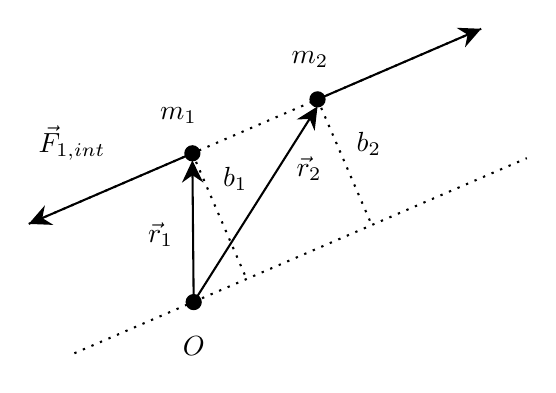
\begin{tikzpicture}[x=0.75pt,y=0.75pt,yscale=-1,xscale=1]
	%uncomment if require: \path (0,300); %set diagram left start at 0, and has height of 300

	%Straight Lines [id:da7593915250022287] 
	\draw  [dash pattern={on 0.84pt off 2.51pt}]  (118.5,205) -- (336.5,111) ;
	%Straight Lines [id:da330620271995024] 
	\draw [line width=0.75]    (121.25,203.81) -- (197.35,171) ;
	\draw [shift={(118.5,205)}, rotate = 336.67] [fill={rgb, 255:red, 0; green, 0; blue, 0 }  ][line width=0.08]  [draw opacity=0] (10.72,-5.15) -- (0,0) -- (10.72,5.15) -- (7.12,0) -- cycle    ;
	%Straight Lines [id:da6426180835226845] 
	\draw [line width=0.75]    (257.65,145) -- (333.75,112.19) ;
	\draw [shift={(336.5,111)}, rotate = 516.6700000000001] [fill={rgb, 255:red, 0; green, 0; blue, 0 }  ][line width=0.08]  [draw opacity=0] (10.72,-5.15) -- (0,0) -- (10.72,5.15) -- (7.12,0) -- cycle    ;
	%Shape: Circle [id:dp1763812532155713] 
	\draw  [fill={rgb, 255:red, 0; green, 0; blue, 0 }  ,fill opacity=1 ] (193.95,171) .. controls (193.95,169.12) and (195.47,167.6) .. (197.35,167.6) .. controls (199.23,167.6) and (200.75,169.12) .. (200.75,171) .. controls (200.75,172.88) and (199.23,174.4) .. (197.35,174.4) .. controls (195.47,174.4) and (193.95,172.88) .. (193.95,171) -- cycle ;
	%Shape: Circle [id:dp8887216402681932] 
	\draw  [fill={rgb, 255:red, 0; green, 0; blue, 0 }  ,fill opacity=1 ] (254.25,145) .. controls (254.25,143.12) and (255.77,141.6) .. (257.65,141.6) .. controls (259.53,141.6) and (261.05,143.12) .. (261.05,145) .. controls (261.05,146.88) and (259.53,148.4) .. (257.65,148.4) .. controls (255.77,148.4) and (254.25,146.88) .. (254.25,145) -- cycle ;
	%Shape: Circle [id:dp7130126320472034] 
	\draw  [fill={rgb, 255:red, 0; green, 0; blue, 0 }  ,fill opacity=1 ] (194.58,242.67) .. controls (194.58,240.79) and (196.11,239.27) .. (197.98,239.27) .. controls (199.86,239.27) and (201.38,240.79) .. (201.38,242.67) .. controls (201.38,244.54) and (199.86,246.07) .. (197.98,246.07) .. controls (196.11,246.07) and (194.58,244.54) .. (194.58,242.67) -- cycle ;
	%Straight Lines [id:da4643521475870709] 
	\draw [line width=0.75]    (197.98,242.67) -- (197.38,177.4) ;
	\draw [shift={(197.35,174.4)}, rotate = 449.47] [fill={rgb, 255:red, 0; green, 0; blue, 0 }  ][line width=0.08]  [draw opacity=0] (10.72,-5.15) -- (0,0) -- (10.72,5.15) -- (7.12,0) -- cycle    ;
	%Straight Lines [id:da7200382141356945] 
	\draw  [dash pattern={on 0.84pt off 2.51pt}]  (140.5,267.33) -- (358.5,173.33) ;
	%Straight Lines [id:da5773842074758675] 
	\draw [line width=0.75]    (197.98,242.67) -- (256.04,150.93) ;
	\draw [shift={(257.65,148.4)}, rotate = 482.33] [fill={rgb, 255:red, 0; green, 0; blue, 0 }  ][line width=0.08]  [draw opacity=0] (10.72,-5.15) -- (0,0) -- (10.72,5.15) -- (7.12,0) -- cycle    ;
	%Shape: Boxed Line [id:dp6958853312388102] 
	\draw  [dash pattern={on 0.84pt off 2.51pt}]  (257.65,145) -- (284.1,206.33) ;
	%Shape: Boxed Line [id:dp6136755725042817] 
	\draw  [dash pattern={on 0.84pt off 2.51pt}]  (197.35,171) -- (223.8,232.33) ;

	% Text Node
	\draw (139.33,166) node    {$\vec{F}_{1,int}$};
	% Text Node
	\draw (182,210.27) node    {$\vec{r}_{1}$};
	% Text Node
	\draw (254,126) node    {$m_{2}$};
	% Text Node
	\draw (190.67,152.67) node    {$m_{1}$};
	% Text Node
	\draw (198,264) node    {$O$};
	% Text Node
	\draw (253.6,178.4) node    {$\vec{r}_{2}$};
	% Text Node
	\draw (282.4,166.4) node    {$b_{2}$};
	% Text Node
	\draw (218,183.33) node    {$b_{1}$};

	\end{tikzpicture}
\end{figure}
\FloatBarrier
L'altra genera un momento in verso orario. Le due forze danno luogo a momenti uguali in modulo e opposti in verso. Per ogni coppia di forze, i momenti delle forze interne sono sempre uguali a zero. Abbiamo quindi ottenuto che

\[
\vec M_\text{tot}^{(o)}=\vec M_\text{tot}^{\text{ext},(o)}=\frac{d\vec L_\text{tot}^{(o)}}{dt}+\vec v_0 \times \vec p_\text{tot}
\]

Il termine ~\eqref{ciao} è zero se come polo si sceglie il centro di massa, oppure se c'è un polo che si muove con velocità parallela al centro di massa o se esso è fisso nel sistema di riferimento inerziale. Questa equazione

\[
	\boxed{\vec{M}_\text{tot}^\text{ext,(o)}=\frac{d\vec{L}_\text{tot}^{(o)}}{dt}}
\]
è nota come \textbf{seconda equazione cardinale della dinamica}. Le forze esterne sono applicate a punti diversi, quindi calcolandone il momento si hanno bracci vettori diversi e non si può dire che il momento della risultante è uguale alla risultante dei momenti.

Per capire l'affermazione:

\[
	\vec{R}_\text{ext}=0 \notimplies \vec{M}_\text{tot}^\text{ext,(o)}=0
\]

si pensi alla ruota di una bicicletta.

\begin{figure}[htpb]
	\centering

	\tikzset{every picture/.style={line width=0.75pt}} %set default line width to 0.75pt        

	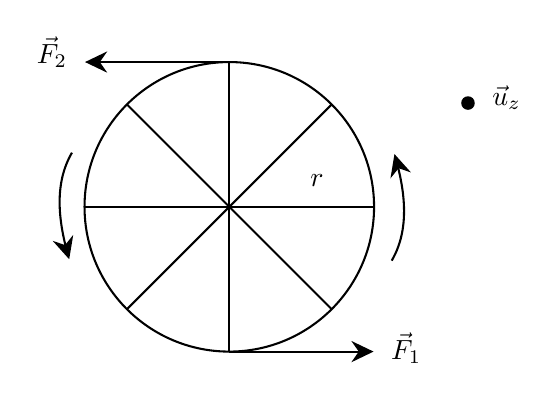
\begin{tikzpicture}[x=0.75pt,y=0.75pt,yscale=-1,xscale=1]
	%uncomment if require: \path (0,300); %set diagram left start at 0, and has height of 300

	%Shape: Circle [id:dp4404111454676727] 
	\draw   (134,158.75) .. controls (134,120.23) and (165.23,89) .. (203.75,89) .. controls (242.27,89) and (273.5,120.23) .. (273.5,158.75) .. controls (273.5,197.27) and (242.27,228.5) .. (203.75,228.5) .. controls (165.23,228.5) and (134,197.27) .. (134,158.75) -- cycle ;
	%Straight Lines [id:da9995352945073703] 
	\draw    (134,158.75) -- (273.5,158.75) ;
	%Straight Lines [id:da3033281097064129] 
	\draw    (203.75,89) -- (203.75,228.5) ;
	%Straight Lines [id:da2400256208242031] 
	\draw    (154.43,109.43) -- (253.07,208.07) ;
	%Straight Lines [id:da6171032237559488] 
	\draw    (253.07,109.43) -- (154.43,208.07) ;
	%Straight Lines [id:da9767183926970966] 
	\draw    (203.75,228.5) -- (270.25,228.5) ;
	\draw [shift={(273.25,228.5)}, rotate = 180] [fill={rgb, 255:red, 0; green, 0; blue, 0 }  ][line width=0.08]  [draw opacity=0] (10.72,-5.15) -- (0,0) -- (10.72,5.15) -- (7.12,0) -- cycle    ;
	%Straight Lines [id:da2493252744323593] 
	\draw    (137.25,89) -- (203.75,89) ;
	\draw [shift={(134.25,89)}, rotate = 0] [fill={rgb, 255:red, 0; green, 0; blue, 0 }  ][line width=0.08]  [draw opacity=0] (10.72,-5.15) -- (0,0) -- (10.72,5.15) -- (7.12,0) -- cycle    ;
	%Curve Lines [id:da3859918903211981] 
	\draw    (282,184.67) .. controls (290.82,169.55) and (288.33,151.45) .. (284.09,136) ;
	\draw [shift={(283.33,133.33)}, rotate = 433.74] [fill={rgb, 255:red, 0; green, 0; blue, 0 }  ][line width=0.08]  [draw opacity=0] (10.72,-5.15) -- (0,0) -- (10.72,5.15) -- (7.12,0) -- cycle    ;
	%Shape: Boxed Bezier Curve [id:dp7410834647628459] 
	\draw    (127.94,132.67) .. controls (119.12,147.79) and (121.61,165.88) .. (125.85,181.33) ;
	\draw [shift={(126.61,184)}, rotate = 253.74] [fill={rgb, 255:red, 0; green, 0; blue, 0 }  ][line width=0.08]  [draw opacity=0] (10.72,-5.15) -- (0,0) -- (10.72,5.15) -- (7.12,0) -- cycle    ;
	%Shape: Circle [id:dp20185600318945807] 
	\draw  [fill={rgb, 255:red, 0; green, 0; blue, 0 }  ,fill opacity=1 ] (316,108.75) .. controls (316,107.23) and (317.23,106) .. (318.75,106) .. controls (320.27,106) and (321.5,107.23) .. (321.5,108.75) .. controls (321.5,110.27) and (320.27,111.5) .. (318.75,111.5) .. controls (317.23,111.5) and (316,110.27) .. (316,108.75) -- cycle ;

	% Text Node
	\draw (246,146) node    {$r$};
	% Text Node
	\draw (289,227) node    {$\vec{F}_{1}$};
	% Text Node
	\draw (118.33,84.33) node    {$\vec{F}_{2}$};
	% Text Node
	\draw (337.33,106.33) node    {$\vec{u}_{z}$};

	\end{tikzpicture}
\end{figure}
\FloatBarrier
Il sistema è costituito da tutte le masse che vanno ad appoggiarsi su di essa.  Si applicano dall'esterno due forze uguali e contrarie in modo che la bicicletta si metta a ruotare. Questo è un esempio in cui la risultante delle forze esterne è zero, ma i momenti delle forze si sommano e si ha:

\[
	\begin{cases} \vec{M}_1=Fr\vec{u}_z \\ \vec{M}_2=Fr\vec{u}_z \end{cases} \implies \vec{M}_\text{tot}=2Fr\vec{u}_z
\]

Il momento totale è diverso da zero perché le forze non giacciono sulla stessa retta di applicazione e hanno quindi la caratteristica di non far traslare il sistema ma di farlo ruotare.

Si capisce quindi come la prima equazione cardinale della dinamica permetta di studiare il moto del centro di massa, mentre la seconda parla del moto rotativo di tutti gli altri punti rispetto ad esso. Le due equazioni sono indipendenti.

Se sul sistema agiscono delle forze che non danno luogo a un momento rispetto al polo $O$, si ha anche in questo caso un principio di conservazione.

\paragraph{Esempio} Si consideri la bacchetta di una majorette che ruota con una certa velocità angolare $\vec{\omega}_0$.

\begin{figure}[htpb]
	\centering

	\tikzset{every picture/.style={line width=0.75pt}} %set default line width to 0.75pt        

	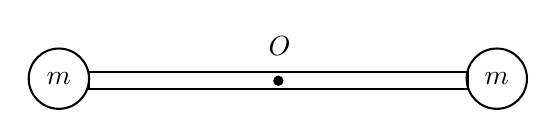
\begin{tikzpicture}[x=0.75pt,y=0.75pt,yscale=-1,xscale=1]
	%uncomment if require: \path (0,300); %set diagram left start at 0, and has height of 300

	%Shape: Rectangle [id:dp3822716726396491] 
	\draw   (134.5,130) -- (317,130) -- (317,138) -- (134.5,138) -- cycle ;
	%Shape: Circle [id:dp8453822070451111] 
	\draw  [fill={rgb, 255:red, 0; green, 0; blue, 0 }  ,fill opacity=1 ] (223.79,134) .. controls (223.79,132.92) and (224.67,132.04) .. (225.75,132.04) .. controls (226.83,132.04) and (227.71,132.92) .. (227.71,134) .. controls (227.71,135.08) and (226.83,135.96) .. (225.75,135.96) .. controls (224.67,135.96) and (223.79,135.08) .. (223.79,134) -- cycle ;

	% Text Node
	\draw    (120, 133) circle [x radius= 14.53, y radius= 14.53]   ;
	\draw (120,133) node    {$m$};
	% Text Node
	\draw    (331, 133) circle [x radius= 14.53, y radius= 14.53]   ;
	\draw (331,133) node    {$m$};
	% Text Node
	\draw (226.29,117.43) node    {$O$};

	\end{tikzpicture}
\end{figure}
\FloatBarrier
Poi la bacchetta, che era inizialmente lunga $2d$, per un meccanismo interno che fa scattare una molla, si allunga del doppio. La domanda che ci si pone (trascurando tutti gli attriti) è quale sia la velocità angolare di rotazione dopo lo scatto del meccanismo interno che ha fatto allungare l'asta. Nel sistema, le forze esterne sono pari a $0$, perché forza peso e reazione normale si bilanciano. Si può affermare che in questo caso i momenti delle forze esterne sono uguali a zero e quindi il momento angolare totale del sistema sarà costante. Si deve conservare il momento angolare, non la velocità angolare.

\begin{gather*}
	\vec{R}_\text{ext}=\frac{d\vec{p}_\text{tot}}{dt} =M_\text{tot}\vec{a}_\text{CM} \\
	\vec{M}_\text{tot}^\text{ext, (o)}=\frac{d\vec{L}_\text{tot}}{dt} \quad \vec{M}_\text{tot}^\text{ext}=0 \implies \vec{L}_\text{tot}^{(o)}=\text{cost}
\end{gather*}

Spostando più massa lontano dal centro di rotazione,  gli oggetti hanno velocità lineare maggiore a parità di $\omega$. Ma $v$ non può variare quindi deve diminuire $\omega$, per permettere al momento angolare di conservarsi.

\begin{gather*}
	\norm{v}=\omega_0 D \quad \vec{L}_\text{tot, in}=\omega_0 D^2m\vec{u}_z+\omega_0 D^2m\vec{u}_z=2\omega_0 D^2m\vec{u}_z \\
	\vec{L}_\text{tot, fin}=m4D^2\omega_\text{fin}\vec{u}_z+m4D^2\omega_\text{fin}\vec{u}_z=8mD^2\omega_\text{fin}\vec{u}_z \\
	2\omega_0 D^2m\vec{u}_z= 8mD^2\omega_\text{fin}\vec{u}_z \implies \omega_\text{fin}=\frac{\omega_0}{4}
\end{gather*}

\section{Teorema dell'energia cinetica}

Si vuole trovare una relazione complessiva che dà l'effetto di tutte le forze sulla variazione di energia cinetica totale del sistema. Si va allora a definire un'altra grandezza complessiva, l'\textbf{energia cinetica totale}:

\[
	E_\text{k, tot}=\sum_{i=1}^nE_{k, i}=\Delta E_\text{k, i}
\]

\begin{equation}
	\label{A}
	\mathcal{L}=\Delta E_k
\end{equation}

Scriviamo la relazione ~\eqref{A} per la generica massa $i-$esima distinguendo forze esterne e interne:

\[
	\mathcal{L}_i^\text{est}+\mathcal{L}_i^\text{int}=\Delta E_{k, i}
\]

Sommando membro a membro si ottiene:

\[
	\boxed{\sum_{i=1}^n \mathcal{L}_i^\text{int}+\sum_{i=1}^n\mathcal{L}_i^\text{est}=\sum_{i=1}^n \Delta E_{k, i}= \Delta E_\text{k, tot}  \quad \text{Teorema dell'energia cinetica}}
\]

La somma dei lavori di tutte le forze esterne daranno luogo a un lavoro che in generale non è nullo e si può andare a calcolare. È evidente che se le traiettorie su cui si muovono le singole masse sono diverse, il termine non va a zero. Questo è il \textbf{teorema dell'energia cinetica} per sistemi di punti materiali, il quale afferma che l'energia cinetica può variare il suo lavoro sia a causa delle forze esterne che a causa delle forze interne.

Si può definire l'\textbf{energia meccanica totale} come somma dell'energia meccanica di ogni punto del sistema, essa varia secondo la relazione:

\[
	\Delta E_\text{mecc}=\mathcal{L}^\text{n.c.}_\text{int}+\mathcal{L}^\text{n.c.}_\text{est}
\]

\paragraph{Esempio} Si immagini di avere un cuneo di massa $M$ su cui è possibile appoggiare un oggetto che può scivolarci sopra. Il piano d'appoggio è perfettamente liscio.

\begin{figure}[htpb]
	\centering

	\tikzset{every picture/.style={line width=0.75pt}} %set default line width to 0.75pt        

	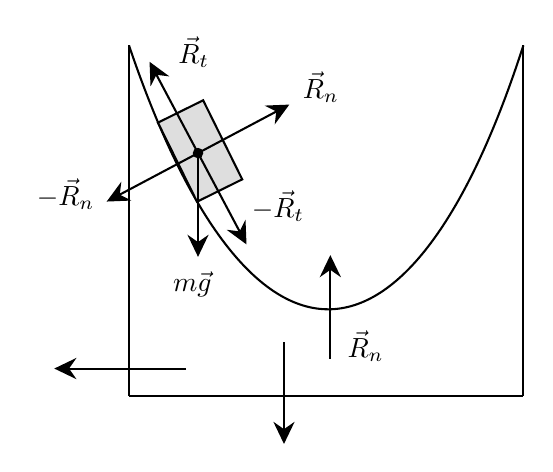
\begin{tikzpicture}[x=0.75pt,y=0.75pt,yscale=-1,xscale=1]
	%uncomment if require: \path (0,300); %set diagram left start at 0, and has height of 300

	%Curve Lines [id:da08474185160861603] 
	\draw    (99,86) .. controls (156.5,256) and (234.5,255) .. (289,86) ;
	%Straight Lines [id:da3600402848302091] 
	\draw    (99,86) -- (99,255) ;
	%Straight Lines [id:da9890701156002613] 
	\draw    (289,86) -- (289,255) ;
	%Straight Lines [id:da14088227593390834] 
	\draw    (99,255) -- (289,255) ;
	%Straight Lines [id:da20165149083647327] 
	\draw    (196,237) -- (196,190) ;
	\draw [shift={(196,187)}, rotate = 450] [fill={rgb, 255:red, 0; green, 0; blue, 0 }  ][line width=0.08]  [draw opacity=0] (10.72,-5.15) -- (0,0) -- (10.72,5.15) -- (7.12,0) -- cycle    ;
	%Straight Lines [id:da3591981245258391] 
	\draw    (173.67,229) -- (173.67,275) ;
	\draw [shift={(173.67,278)}, rotate = 270] [fill={rgb, 255:red, 0; green, 0; blue, 0 }  ][line width=0.08]  [draw opacity=0] (10.72,-5.15) -- (0,0) -- (10.72,5.15) -- (7.12,0) -- cycle    ;
	%Straight Lines [id:da5542442706390196] 
	\draw    (126.5,241.67) -- (66,241.67) ;
	\draw [shift={(63,241.67)}, rotate = 360] [fill={rgb, 255:red, 0; green, 0; blue, 0 }  ][line width=0.08]  [draw opacity=0] (10.72,-5.15) -- (0,0) -- (10.72,5.15) -- (7.12,0) -- cycle    ;
	%Shape: Rectangle [id:dp24134016790920998] 
	\draw  [fill={rgb, 255:red, 222; green, 222; blue, 222 }  ,fill opacity=1 ] (134.72,112.43) -- (153.55,150.52) -- (131.78,161.29) -- (112.95,123.19) -- cycle ;
	%Straight Lines [id:da1394008418051096] 
	\draw    (132.25,137.86) -- (173.6,115.91) ;
	\draw [shift={(176.25,114.5)}, rotate = 512.04] [fill={rgb, 255:red, 0; green, 0; blue, 0 }  ][line width=0.08]  [draw opacity=0] (10.72,-5.15) -- (0,0) -- (10.72,5.15) -- (7.12,0) -- cycle    ;
	%Straight Lines [id:da12135194002047722] 
	\draw    (90.9,159.81) -- (132.25,137.86) ;
	\draw [shift={(88.25,161.21)}, rotate = 332.04] [fill={rgb, 255:red, 0; green, 0; blue, 0 }  ][line width=0.08]  [draw opacity=0] (10.72,-5.15) -- (0,0) -- (10.72,5.15) -- (7.12,0) -- cycle    ;
	%Straight Lines [id:da11104915980985175] 
	\draw    (132.25,184.86) -- (132.25,137.86) ;
	\draw [shift={(132.25,187.86)}, rotate = 270] [fill={rgb, 255:red, 0; green, 0; blue, 0 }  ][line width=0.08]  [draw opacity=0] (10.72,-5.15) -- (0,0) -- (10.72,5.15) -- (7.12,0) -- cycle    ;
	%Shape: Circle [id:dp285260685691167] 
	\draw  [fill={rgb, 255:red, 0; green, 0; blue, 0 }  ,fill opacity=1 ] (130.25,137.86) .. controls (130.25,136.75) and (131.15,135.86) .. (132.25,135.86) .. controls (133.35,135.86) and (134.25,136.75) .. (134.25,137.86) .. controls (134.25,138.96) and (133.35,139.86) .. (132.25,139.86) .. controls (131.15,139.86) and (130.25,138.96) .. (130.25,137.86) -- cycle ;
	%Shape: Boxed Line [id:dp8945452096934903] 
	\draw    (132.25,137.86) -- (154.2,179.21) ;
	\draw [shift={(155.61,181.86)}, rotate = 242.04] [fill={rgb, 255:red, 0; green, 0; blue, 0 }  ][line width=0.08]  [draw opacity=0] (10.72,-5.15) -- (0,0) -- (10.72,5.15) -- (7.12,0) -- cycle    ;
	%Straight Lines [id:da9166808228451746] 
	\draw    (110.3,96.51) -- (132.25,137.86) ;
	\draw [shift={(108.89,93.86)}, rotate = 62.04] [fill={rgb, 255:red, 0; green, 0; blue, 0 }  ][line width=0.08]  [draw opacity=0] (10.72,-5.15) -- (0,0) -- (10.72,5.15) -- (7.12,0) -- cycle    ;

	% Text Node
	\draw (213,230.67) node    {$\vec{R}_{n}$};
	% Text Node
	\draw (191.5,106) node    {$\vec{R}_{n}$};
	% Text Node
	\draw (68.5,157.5) node    {$-\vec{R}_{n}$};
	% Text Node
	\draw (129.5,201) node    {$m\vec{g}$};
	% Text Node
	\draw (130.17,89.33) node    {$\vec{R}_{t}$};
	% Text Node
	\draw (170.83,163.33) node    {$-\vec{R}_{t}$};

	\end{tikzpicture}
\end{figure}
\FloatBarrier
Se l'oggetto parte da fermo, quello che accade è che tenderà a scivolare a causa dell'effetto della forza peso ed è naturale pensare che se non c'è attrito, esso, partendo da fermo, trasformerà la sua energia potenziale in energia cinetica che poi, ripartendo verso l'alto, si ritrasformerà in energia potenziale. L'oggetto oscillerà sul cuneo. A causa del fatto che questo si sta muovendo complessivamente verso destra, ci si aspetta che il cuneo dovrà partire verso sinistra per la conservazione della quantità di moto. Dal punto di vista delle forze esterne, agiscono il peso e la reazione normale al piano d'appoggio, tutte in direzione verticale.

Le forze totali esterne sono $0$ in direzione $x$ e questo comporta che la quantità di moto totale del sistema valutata in tale direzione dovrà essere costante. Il sistema inizialmente aveva quantità di moto iniziale zero, quindi essa si deve continuare a mantenere tale: l'ascissa del centro di massa non deve variare nel tempo. Quando la massa si sposta verso destra il cuneo, per compensare, si sposta a sinistra. Se per assurdo la massa si spostasse e arrivasse dall'altra parte senza che il cuneo si muovesse, il centro di massa si sposterebbe in basso. Da un punto di vista fisico, ciò che fa spostare il cuneo è l'effetto di una forza interna. La reazione normale sull'oggetto è generata dal cuneo; allora la massa $m$ genererà su di esso una forza uguale e contraria.

Si immagini di complicare la situazione avendo la forza d'attrito, interna, che rallenta il movimento. Il suo effetto è nullo nel valutare la prima equazione cardinale della dinamica. Ma dal punto di vista energetico queste forze interne hanno un effetto. L'attrito va a dissipare l'energia potenziale, così che l'oggetto arriverà al lato opposto del cuneo a quote via via inferiori. Quest'ultimo subirà una forza $-\vec{R}_n$ e $-\vec{R}_t$. L'oggetto scivolerà verso il basso. Ma è come se si muovesse su un sistema di riferimento relativo che trasla, perché il cuneo si muove. $\vec{R}_t$, $-\vec{R}_t$ si elidono. Vale lo stesso per $\vec{R}_n$ e $-\vec{R}_n$. Il calcolo del lavoro è il lavoro della forza d'attrito valutata su tutto lo spostamento del cuneo. Si noti infatti che il cuneo e la massa seguono traiettorie diverse quindi, benché $\vec{R}_t$ e $-\vec{R}_t$ siano uguali ed opposte, il loro lavoro è valutato su una traiettoria differente.

\section{Urti tra due punti materiali}

\[
	\vec{R}_\text{est}=\frac{d\vec{p}_\text{tot}}{dt} \qquad \Delta E_k=\mathcal{L}_\text{int}+\mathcal{L}_\text{est} \qquad \vec{M}_\text{tot}=\frac{d\vec{L}_\text{tot}}{dt}
\]

Queste sono le tre relazioni che possono aiutare nello studio del moto di un sistema di punti. Un esempio tipico di applicazione di ciò è lo studio del fenomeno di urto fra punti.

Quando due punti materiali vengono a contatto e interagiscono per un intervallo di tempo trascurabile rispetto a quello di osservazione del sistema, si parla di \textbf{urto} tra due punti. È evidente che quando due corpi si scontrano, entrano in gioco forze interne molto elevate che passano dall'essere nulle prima del fenomeno di urto, all'essere di intensità molto elevate durante tale fenomeno. Studiandone l'andamento nell'intervallo di tempo, si può vedere come esse abbiano un carattere fortemente impulsivo. Le forze esterne invece si mantengono per lo più costanti durante il fenomeno di urto e se variano variano molto poco il proprio valore. Inoltre esse sono in generale molto meno intense rispetto a quelle interne.

\begin{figure}[htpb]
	\centering

	\tikzset{every picture/.style={line width=0.75pt}} %set default line width to 0.75pt        

	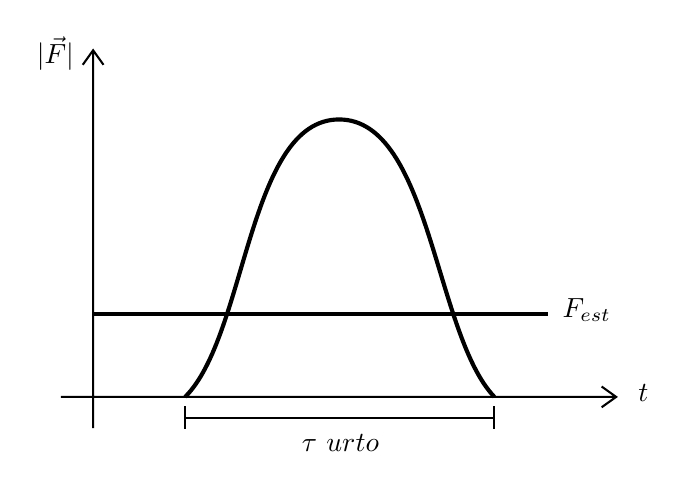
\begin{tikzpicture}[x=0.75pt,y=0.75pt,yscale=-1,xscale=1]
	%uncomment if require: \path (0,300); %set diagram left start at 0, and has height of 300

	%Shape: Axis 2D [id:dp9573824779450613] 
	\draw  (50.67,220) -- (318.17,220)(66.17,53) -- (66.17,235) (311.17,215) -- (318.17,220) -- (311.17,225) (61.17,60) -- (66.17,53) -- (71.17,60)  ;
	%Curve Lines [id:da6395267149757182] 
	\draw [line width=1.5]    (110.5,220) .. controls (140.25,190.5) and (140.67,86.33) .. (184.67,86.33) .. controls (228.67,86.33) and (230.75,190) .. (259.5,220) ;
	%Straight Lines [id:da8778937063159087] 
	\draw    (110.5,230) -- (259.5,230) ;
	\draw [shift={(259.5,230)}, rotate = 180] [color={rgb, 255:red, 0; green, 0; blue, 0 }  ][line width=0.75]    (0,5.59) -- (0,-5.59)   ;
	\draw [shift={(110.5,230)}, rotate = 180] [color={rgb, 255:red, 0; green, 0; blue, 0 }  ][line width=0.75]    (0,5.59) -- (0,-5.59)   ;
	%Straight Lines [id:da4441851887710484] 
	\draw [line width=1.5]    (66.17,180) -- (285.17,180) ;

	% Text Node
	\draw (48,54.67) node    {$|\vec{F} |$};
	% Text Node
	\draw (331.33,218) node    {$t$};
	% Text Node
	\draw (185.33,242) node    {$\tau \ \text{urto}$};
	% Text Node
	\draw (304,178) node    {$F_{\text{est}}$};

	\end{tikzpicture}
\end{figure}
\FloatBarrier
Si va a riscrivere la prima equazione cardinale della dinamica in termini di teorema dell'impulso. I corpi che si urtano diventano il sistema di corpi.

\[
	\int_0^\tau \vec{R}_\text{est}\,dt=\Delta \vec{p}_\text{tot}
\]

Se l'intervallo di tempo è molto molto piccolo, tale per cui può essere approssimato a zero, il primo termine va a 0: ciò comporta che durante questi fenomeni la quantità di moto del sistema si mantiene costante. Allora, il moto del centro di massa non viene alterato dall'urto. Analogamente si può attuare la stessa osservazione per la seconda equazione cardinale della dinamica: i momenti delle forze esterne durante l'urto hanno un effetto praticamente nullo e quindi il momento angolare totale rispetto a un qualunque polo $O$ del sistema è costante durante il fenomeno.

\[
	\int_0^\tau \vec{M}_\text{est}\,dt=\Delta \vec{L}^{(o)} \implies \vec{L}_\text{tot}=\text{cost}
\]

Quando i fenomeni di urto interessano un sistema che ruota è utile questa relazione. In una situazione di urto, i punti si movono verso il centro di massa ed entrano in contatto in corrispondenza di esso.

Infine è possibile attuare delle considerazione energetiche. Ci si chiede se e come varia l'energia totale del sistema durante i fenomeni di urto. In questo caso bisogna tenere conto del fatto che le forze interne, che hanno intensità molto elevata, entrano in gioco nel far variare l'energia totale del sistema. Se ci sono forze non conservative l'energia totale varia. Le forze esterne si possono di nuovo trascurare, ciò che però è interessante notare è che l'effetto dissipativo delle forze interne fa variare l'energia cinetica del sistema. La variazione di energia potenziale è all'incirca zero. È infatti un'energia posizionale che dà un valore a seconda della posizione dei corpi, ma il fenomeno è di così breve durata da giustificare l'assunzione che durante l'interazione i punti non si muovono in modo apprezzabile.

\[
	\mathcal{L}_\text{int}^\text{NC}+\mathcal{L}_\text{est}^\text{NC}=\Delta E_\text{mecc}=\Delta E_\text{k, tot}+\underbrace{\Delta E_\text{p, tot}}_{=0}
\]

Quindi se ci sono forze interne dissipative queste vanno a variare l'energia cinetica totale del sistema.

\subsection{Urti elastici e anelastici}

Dal punto di vista energetico, si possono distinguere gli urti in due grandi tipologie: urti \textbf{ideali} o \textbf{elastici}, in cui le forze interne sono tutte conservative, e quindi non si ha effetto di dissipazione per causa loro, e urti \textbf{anelastici}.

\paragraph{Urti elastici} Si definisce come urto elastico un urto durante il quale si conserva anche l'energia cinetica del sistema. Questo comporta che le forze interne, che si manifestano durante l'urto, siano conservative. I due corpi reali che si urtano subiscono, durante l'urto, delle deformazioni elastiche, riprendendo la configurazione iniziale subito dopo di esso.
Il termine:

\[
	\mathcal{L}_\text{int}^\text{NC}=\Delta E_\text{k, tot}
\]

Va a zero e l'energia totale del sistema è costante.
Nello studio di un sistema elastico si possono utilizzare quindi le equazioni:

\[
	P_\text{in}=P_\text{fin} \quad E_\text{k, in}=E_\text{k, fin}
\]

Si pensi all'urto tra palle da biliardo, le forze che si scambiano durante l'urto non variano l'energia del sistema e si osserva trasferimento di energia cinetica da un corpo all'altro.

\paragraph{Urti anelastici} Si tratta di urti che avvengono in presenza di forze interne non conservative con conseguente variazione di energia cinetica durante il fenomeno. Questa seconda classe rappresenta la vera categoria degli urti, la prima è principalmente un'idealizzazione. Se le forze interne sono dissipative l'energia cinetica diminuirà, anche se ci sono casi in cui le forze interne possono far aumentare l'energia del sistema.

\paragraph{Urto completamente anelastico} Tra gli urti anelastici, si trova una sottoclasse di fenomeni di urto che prende il nome di \textbf{urti completamente anelastici}: sono quei fenomeni di urto in cui i corpi che si sono urtati dopo l'evento rimangono insieme, formando un unico corpo puntiforme di massa $m_1+m_2$ che si muove con una certa velocità finale. Per far unire i corpi insieme devono aver agito forze interne che hanno dissipato l'energia cinetica. I due corpi, che si assimilano a punti materiali, durante l'urto si deformano in modo permanente e restano compenetrati. Il lavoro compiuto, a spese dell'energia cinetica iniziale, per fare avvenire la deformazione, non viene più recuperato, cosa che equivale ad affermare che le forze interne sviluppate nell'atto non sono conservative. Inoltre, dopo l'urto completamente anelastico, non c'è più moto rispetto al centro di massa.

\subsection{Urti centrali e non centrali}

Gli urti si classificano anche in centrali e non centrali.

\paragraph{Urti centrali} Gli urti \textbf{centrali} sono quei fenomeni di urto in cui i corpi interessati viaggiano in una certa direzione e dopo il fenomeno continuano a viaggiare nella stessa direzione (anche se il verso può essere opposto). In pratica gli urti centrali sono semplici da studiare perché dal punto di vista della quantità di moto il problema vettoriale è monodimensionale. Si osserva il tutto nell'unica direzione in cui avviene l'urto.

\paragraph{Urti non centrali} Gli urti \textbf{non centrali} sono invece quelli che avvengono non nella stessa direzione. I corpi possono avere dopo di essi una direzione qualunque.

L'obbiettivo dello studio del fenomeno di urto è ricavare la velocità dei due corpi dopo di esso. In \textit{urti centrali elastici}, in cui le forze esterne non sono impulsive, si conserva la quantità di moto totale del sistema. Essendo elastico, l'energia cinetica totale del sistema è costante.

\begin{gather*}
	p_\text{tot}=\text{cost} \quad m_1 v_1+m_2 v_2=m_1 v_{1,\text{fin}}+m_2 v_{2,\text{fin}} \\
	E_\text{k, tot}=\text{cost} \quad \frac{1}{2}m_1 v_1^2+\frac{1}{2}m_2 v_2^2=\frac{1}{2}m_1 v_{1,\text{fin}}^2+\frac{1}{2}m_2 v_{2,\text{fin}}^2
\end{gather*}

Si hanno due incognite, il problema è risolvibile.

\begin{gather*}
	v_{1,\text{fin}}=\frac{m_1-m_2}{m_1+m_2} v_1+\underbrace{\frac{2m_2 v_2}{m_1+m_2}}_A \\
	v_{2,\text{fin}}=\frac{2m_1 v_1}{m_1+m_2}+\underbrace{\frac{m_2-m_1 v_2}{m_1+m_2}}_B
\end{gather*}

\begin{figure}[htpb]
	\centering

	\tikzset{every picture/.style={line width=0.75pt}} %set default line width to 0.75pt        

	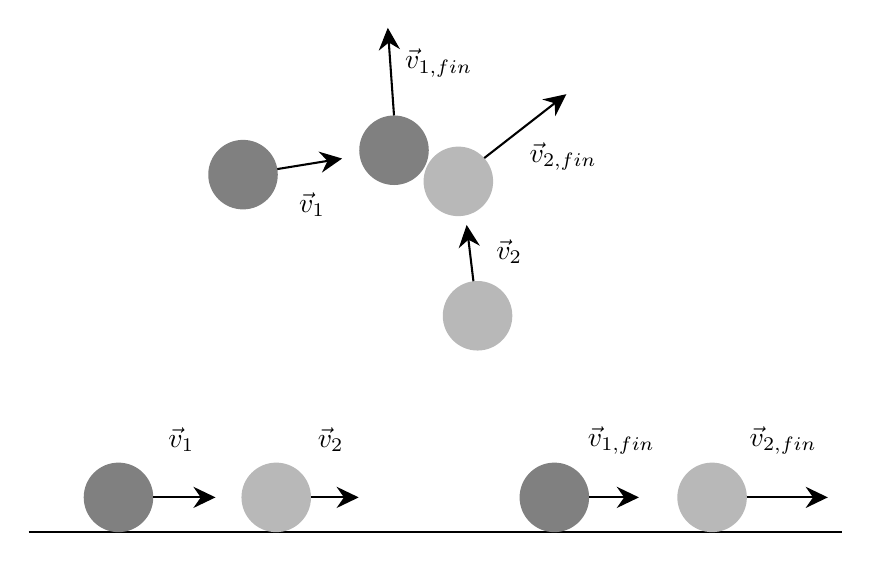
\begin{tikzpicture}[x=0.75pt,y=0.75pt,yscale=-1,xscale=1]
	%uncomment if require: \path (0,392); %set diagram left start at 0, and has height of 392

	%Straight Lines [id:da23785241410349744] 
	\draw    (118.75,106.75) -- (163.54,99.48) ;
	\draw [shift={(166.5,99)}, rotate = 530.78] [fill={rgb, 255:red, 0; green, 0; blue, 0 }  ][line width=0.08]  [draw opacity=0] (10.72,-5.15) -- (0,0) -- (10.72,5.15) -- (7.12,0) -- cycle    ;
	%Straight Lines [id:da8050824923621605] 
	\draw    (231.75,174.75) -- (226.86,133.98) ;
	\draw [shift={(226.5,131)}, rotate = 443.16] [fill={rgb, 255:red, 0; green, 0; blue, 0 }  ][line width=0.08]  [draw opacity=0] (10.72,-5.15) -- (0,0) -- (10.72,5.15) -- (7.12,0) -- cycle    ;
	%Shape: Circle [id:dp9455071582439742] 
	\draw  [draw opacity=0][fill={rgb, 255:red, 128; green, 128; blue, 128 }  ,fill opacity=1 ] (102,106.75) .. controls (102,97.5) and (109.5,90) .. (118.75,90) .. controls (128,90) and (135.5,97.5) .. (135.5,106.75) .. controls (135.5,116) and (128,123.5) .. (118.75,123.5) .. controls (109.5,123.5) and (102,116) .. (102,106.75) -- cycle ;
	%Shape: Circle [id:dp34714784890720884] 
	\draw  [draw opacity=0][fill={rgb, 255:red, 184; green, 184; blue, 184 }  ,fill opacity=1 ] (215,174.75) .. controls (215,165.5) and (222.5,158) .. (231.75,158) .. controls (241,158) and (248.5,165.5) .. (248.5,174.75) .. controls (248.5,184) and (241,191.5) .. (231.75,191.5) .. controls (222.5,191.5) and (215,184) .. (215,174.75) -- cycle ;
	%Shape: Circle [id:dp3095792636280448] 
	\draw  [draw opacity=0][fill={rgb, 255:red, 128; green, 128; blue, 128 }  ,fill opacity=1 ] (174.75,95) .. controls (174.75,85.75) and (182.25,78.25) .. (191.5,78.25) .. controls (200.75,78.25) and (208.25,85.75) .. (208.25,95) .. controls (208.25,104.25) and (200.75,111.75) .. (191.5,111.75) .. controls (182.25,111.75) and (174.75,104.25) .. (174.75,95) -- cycle ;
	%Straight Lines [id:da9403834889901768] 
	\draw    (191.5,78.25) -- (188.71,38.99) ;
	\draw [shift={(188.5,36)}, rotate = 445.94] [fill={rgb, 255:red, 0; green, 0; blue, 0 }  ][line width=0.08]  [draw opacity=0] (10.72,-5.15) -- (0,0) -- (10.72,5.15) -- (7.12,0) -- cycle    ;
	%Straight Lines [id:da8870317581239819] 
	\draw    (230.5,102.25) -- (272.13,69.84) ;
	\draw [shift={(274.5,68)}, rotate = 502.1] [fill={rgb, 255:red, 0; green, 0; blue, 0 }  ][line width=0.08]  [draw opacity=0] (10.72,-5.15) -- (0,0) -- (10.72,5.15) -- (7.12,0) -- cycle    ;
	%Shape: Circle [id:dp9617349145835501] 
	\draw  [draw opacity=0][fill={rgb, 255:red, 184; green, 184; blue, 184 }  ,fill opacity=1 ] (205.75,110) .. controls (205.75,100.75) and (213.25,93.25) .. (222.5,93.25) .. controls (231.75,93.25) and (239.25,100.75) .. (239.25,110) .. controls (239.25,119.25) and (231.75,126.75) .. (222.5,126.75) .. controls (213.25,126.75) and (205.75,119.25) .. (205.75,110) -- cycle ;
	%Straight Lines [id:da004649770034952372] 
	\draw    (15.5,279) -- (407.5,279) ;
	%Shape: Circle [id:dp49171906743296834] 
	\draw  [draw opacity=0][fill={rgb, 255:red, 128; green, 128; blue, 128 }  ,fill opacity=1 ] (42,262.25) .. controls (42,253) and (49.5,245.5) .. (58.75,245.5) .. controls (68,245.5) and (75.5,253) .. (75.5,262.25) .. controls (75.5,271.5) and (68,279) .. (58.75,279) .. controls (49.5,279) and (42,271.5) .. (42,262.25) -- cycle ;
	%Shape: Circle [id:dp5105287976415633] 
	\draw  [draw opacity=0][fill={rgb, 255:red, 184; green, 184; blue, 184 }  ,fill opacity=1 ] (118,262.25) .. controls (118,253) and (125.5,245.5) .. (134.75,245.5) .. controls (144,245.5) and (151.5,253) .. (151.5,262.25) .. controls (151.5,271.5) and (144,279) .. (134.75,279) .. controls (125.5,279) and (118,271.5) .. (118,262.25) -- cycle ;
	%Straight Lines [id:da2603449450705637] 
	\draw    (75.5,262.25) -- (102.5,262.25) ;
	\draw [shift={(105.5,262.25)}, rotate = 180] [fill={rgb, 255:red, 0; green, 0; blue, 0 }  ][line width=0.08]  [draw opacity=0] (10.72,-5.15) -- (0,0) -- (10.72,5.15) -- (7.12,0) -- cycle    ;
	%Straight Lines [id:da6285993598469684] 
	\draw    (151.5,262.25) -- (171.5,262.25) ;
	\draw [shift={(174.5,262.25)}, rotate = 180] [fill={rgb, 255:red, 0; green, 0; blue, 0 }  ][line width=0.08]  [draw opacity=0] (10.72,-5.15) -- (0,0) -- (10.72,5.15) -- (7.12,0) -- cycle    ;
	%Shape: Circle [id:dp8061709344353809] 
	\draw  [draw opacity=0][fill={rgb, 255:red, 128; green, 128; blue, 128 }  ,fill opacity=1 ] (252,262.25) .. controls (252,253) and (259.5,245.5) .. (268.75,245.5) .. controls (278,245.5) and (285.5,253) .. (285.5,262.25) .. controls (285.5,271.5) and (278,279) .. (268.75,279) .. controls (259.5,279) and (252,271.5) .. (252,262.25) -- cycle ;
	%Shape: Circle [id:dp4212709157924077] 
	\draw  [draw opacity=0][fill={rgb, 255:red, 184; green, 184; blue, 184 }  ,fill opacity=1 ] (328,262.25) .. controls (328,253) and (335.5,245.5) .. (344.75,245.5) .. controls (354,245.5) and (361.5,253) .. (361.5,262.25) .. controls (361.5,271.5) and (354,279) .. (344.75,279) .. controls (335.5,279) and (328,271.5) .. (328,262.25) -- cycle ;
	%Straight Lines [id:da44241450213871514] 
	\draw    (285.5,262.25) -- (306.5,262.25) ;
	\draw [shift={(309.5,262.25)}, rotate = 180] [fill={rgb, 255:red, 0; green, 0; blue, 0 }  ][line width=0.08]  [draw opacity=0] (10.72,-5.15) -- (0,0) -- (10.72,5.15) -- (7.12,0) -- cycle    ;
	%Straight Lines [id:da8915950053595205] 
	\draw    (361.5,262.25) -- (397.5,262.25) ;
	\draw [shift={(400.5,262.25)}, rotate = 180] [fill={rgb, 255:red, 0; green, 0; blue, 0 }  ][line width=0.08]  [draw opacity=0] (10.72,-5.15) -- (0,0) -- (10.72,5.15) -- (7.12,0) -- cycle    ;

	% Text Node
	\draw (152,121) node    {$\vec{v}_{1}$};
	% Text Node
	\draw (247,144) node    {$\vec{v}_{2}$};
	% Text Node
	\draw (273,98) node    {$\vec{v}_{2,\text{fin}}$};
	% Text Node
	\draw (213,53) node    {$\vec{v}_{1,\text{fin}}$};
	% Text Node
	\draw (89,234.5) node    {$\vec{v}_{1}$};
	% Text Node
	\draw (161,234.5) node    {$\vec{v}_{2}$};
	% Text Node
	\draw (301,235) node    {$\vec{v}_{1,\text{fin}}$};
	% Text Node
	\draw (379,235) node    {$\vec{v}_{2,\text{fin}}$};

	\end{tikzpicture}
\end{figure}
\FloatBarrier
Un caso interessante si ha quando una massa va a urtare un'altra massa inizialmente ferma. Il risultato che si ottiene è lo stesso senza i termini $A$ e $B$. La pallina nel secondo caso parte con velocità identica a quella della prima: si dice che i due corpi si scambiano la quantità di moto.

\[
	v_{1,\text{fin}} \begin{cases}  >0 & \text{se $m_1>m_2$} \\ <0 & \text{se $m_1<m_2$} \\ =0 &\text{se $m_1=m_2$} \end{cases}
\]

Nel caso di \textit{urti centrali anelastici}, si può imporre la conservazione della quantità di moto. Essendo l'urto anelastico, l'energia cinetica del sistema non è costante e varia nel tempo. Come nel caso precedente, si hanno due incognite ma una sola equazione scalare. Quindi non è sufficiente usare la sola conservazione della quantità di moto. Si deve avere un'informazione ad esempio su come è variata l'energia cinetica totale del sistema. Diversa è la situazione se l'urto è completamente anelastico. Si impone infatti di nuovo la conservazione della quantità di moto, ma se l'urto è anelastico completo i corpi si muovono insieme con la stessa velocità, quindi si ha una sola incognita.

Si rimuove ora l'ipotesi che le forze esterne non siano impulsive. In tal caso il loro effetto non è più trascurabile durante l'urto. Si immagini di avere un blocco di massa $M$ su un piano d'appoggio orizzontale.

\begin{figure}[htpb]
	\centering

	\tikzset{every picture/.style={line width=0.75pt}} %set default line width to 0.75pt        

	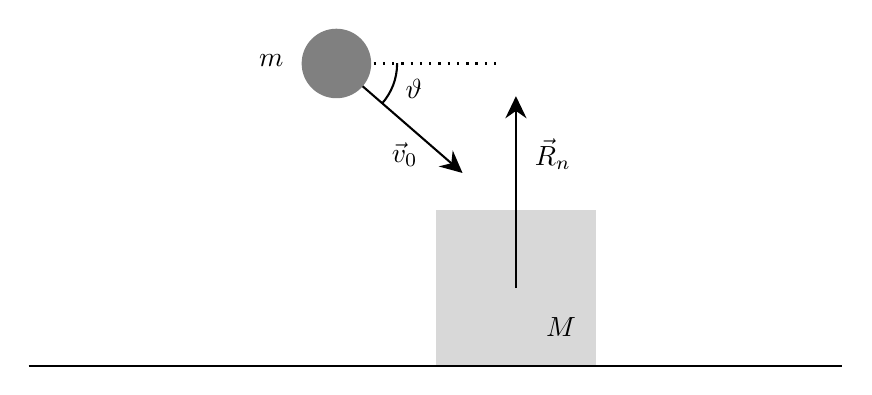
\begin{tikzpicture}[x=0.75pt,y=0.75pt,yscale=-1,xscale=1]
	%uncomment if require: \path (0,300); %set diagram left start at 0, and has height of 300

	%Shape: Rectangle [id:dp12759655748744736] 
	\draw  [draw opacity=0][fill={rgb, 255:red, 216; green, 216; blue, 216 }  ,fill opacity=1 ] (235.5,144) -- (313,144) -- (313,219) -- (235.5,219) -- cycle ;
	%Straight Lines [id:da99326183921629] 
	\draw    (39.5,219) -- (431.5,219) ;
	%Straight Lines [id:da4219217975595948] 
	\draw    (274.25,181.5) -- (274.25,92) ;
	\draw [shift={(274.25,89)}, rotate = 450] [fill={rgb, 255:red, 0; green, 0; blue, 0 }  ][line width=0.08]  [draw opacity=0] (10.72,-5.15) -- (0,0) -- (10.72,5.15) -- (7.12,0) -- cycle    ;
	%Straight Lines [id:da835878792476836] 
	\draw    (187.75,73.25) -- (246.23,124.03) ;
	\draw [shift={(248.5,126)}, rotate = 220.97] [fill={rgb, 255:red, 0; green, 0; blue, 0 }  ][line width=0.08]  [draw opacity=0] (10.72,-5.15) -- (0,0) -- (10.72,5.15) -- (7.12,0) -- cycle    ;
	%Straight Lines [id:da9881246029528177] 
	\draw  [dash pattern={on 0.84pt off 2.51pt}]  (187.75,73.25) -- (267.25,73.25) ;
	%Shape: Arc [id:dp002943181307110132] 
	\draw  [draw opacity=0] (217,73.06) .. controls (217,73.12) and (217,73.19) .. (217,73.25) .. controls (217,80.69) and (214.22,87.49) .. (209.64,92.65) -- (187.75,73.25) -- cycle ; \draw   (217,73.06) .. controls (217,73.12) and (217,73.19) .. (217,73.25) .. controls (217,80.69) and (214.22,87.49) .. (209.64,92.65) ;
	%Shape: Circle [id:dp4761852792534427] 
	\draw  [draw opacity=0][fill={rgb, 255:red, 128; green, 128; blue, 128 }  ,fill opacity=1 ] (171,73.25) .. controls (171,64) and (178.5,56.5) .. (187.75,56.5) .. controls (197,56.5) and (204.5,64) .. (204.5,73.25) .. controls (204.5,82.5) and (197,90) .. (187.75,90) .. controls (178.5,90) and (171,82.5) .. (171,73.25) -- cycle ;

	% Text Node
	\draw (292,117) node    {$\vec{R}_{n}$};
	% Text Node
	\draw (296,200) node    {$M$};
	% Text Node
	\draw (220.67,117.33) node    {$\vec{v}_{0}$};
	% Text Node
	\draw (225,85.67) node    {$\vartheta $};
	% Text Node
	\draw (156.33,72) node    {$m$};

	\end{tikzpicture}
\end{figure}
\FloatBarrier
Su di esso viene lanciato un oggetto di massa $m$ con velocità $v_o$, inclinata di un certo angolo rispetto alla direzione orizzontale. Le forze esterne che agiscono durante l'urto sono la forza peso della massa $m$ e quella della massa $M$ che non variano durante l'urto, ma c'è un altra forza impulsiva: la reazione normale. Essa varia perché quando la pallina va a conficcarsi nell'oggetto di massa $M$,  tende a scaricare una certa forza lungo la verticale, bilanciata dalla reazione normale, che aumenta istantaneamente. Quando agiscono forze esterne che hanno carattere impulsivo, non è più possibile trascurarle e quindi non è più vero che si conserva la quantità di moto totale durante l'urto. La reazione normale ha direzione solo verticale, quindi nella direzione non verticale non agiscono forze esterne impulsive. Il sistema varierà la sua quantità di moto lungo la direzione verticale, ma non lungo quella orizzontale. Si può applicare ancora il principio di conservazione della quantità di moto in una sola direzione. Si immagini che dopo l'urto la massa si conficchi nel corpo di massa $M$: si avrà un sistema di massa complessiva $m+M$ che viaggia in orizzontale con una certa velocità finale incognita. La quantità di moto scomposta in direzione $x$ iniziale si trasforma tutta in quantità di moto finale. La quantità di moto è variata perché la forza in direzione verticale ha assorbito la quantità di moto iniziale.

\begin{gather*}
	p_\text{x, tot}=\text{cost.} \qquad mv_0\cos\vartheta=(m+M)v_\text{fin} \qquad \Delta p_\text{y, tot} \ne 0 \\
	\implies 0+mv_0\sin\vartheta=\int_0^\tau R_n \, dt
\end{gather*}

\section{I teoremi di K\"onig}

Si termina lo studio della dinamica dei sistemi di punti materiali con l'introduzione di due teoremi molto importanti: essi prendono il nome di teoremi di K\"onig. Le grandezze caratteristiche di un sistema di punti materiali che finora sono state definite sono le seguenti:

\begin{itemize}
	\item $\vec{p}_\text{tot}$, quantità di moto complessiva. Si tratta della somma della quantità di moto di ogni singolo punto materiale e fornisce un'informazione su come sta traslando il sistema nel suo complesso.
	\item $\vec{L}_\text{tot}$, momento angolare complessivo rispetto al polo $O$. Esso non è altro che la somma dei momenti angolari posseduti da ogni punto materiale.
	\item $E_\text{k, tot}$, energia cinetica totale. È la somma scalare dell'energia cinetica posseduta da ogni punto materiale.
\end{itemize}

Accanto a queste grandezze è possibile definire quelle analoghe riferite al centro di massa. Se in esso si va a concentrare la massa totale del sistema, si definisce la sua quantità di moto come:

\[
	\vec{p}_\text{CM} = M_\text{tot} \, \vec{v}_\text{CM}
\]

Si può anche definire il \textbf{momento angolare del centro di massa} come:

\[
	\boxed{\vec{L}_\text{CM}^{(o)} = \vec{M}_\text{CM}^{(o)} \times M_{tot} \, \vec{v}_\text{CM}}
\]

Ci si potrebbe chiedere se è possibile descrivere il sistema di punti semplicemente in termini di centro di massa. Per il primo teorema del centro di massa, si sa che la quantità di moto totale del sistema è uguale a quella del solo CM. Si può dire la stessa cosa per l'energia cinetica e il momento angolare? I due teoremi di K\"onig rispondono proprio a questa domanda. Il momento angolare del centro di massa dà informazioni sul fatto che tale punto CM possiede un certo momento angolare, quindi che in qualche maniera sta ruotando attorno al polo $O$. Se il momento angolare del centro di massa è nullo tuttavia non si può affermare che i vari punti del sistema non abbiano alcun momento angolare rispetto a tale polo. Il sistema può ruotare mentre il centro di massa non ha momento angolare, ad esempio perché i corpi stanno ruotando attorno al polo. In tal caso la velocità del CM sarà nulla, ma il sistema possiederà sicuramente una certa energia cinetica perché le sue parti ruotano. È evidente che non ha senso immaginare di descrivere il sistema di punti in termini del solo centro di massa. I teoremi di K\"onig daranno una descrizione di queste due quantità in termini di centro di massa e di una quantità aggiuntiva.

\paragraph{Primo teorema di K\"onig} Si supponga di avere il sistema di punti materiali e un punto fisso $O$.

\begin{figure}[htpb]
	\centering

	\tikzset{every picture/.style={line width=0.75pt}} %set default line width to 0.75pt        

	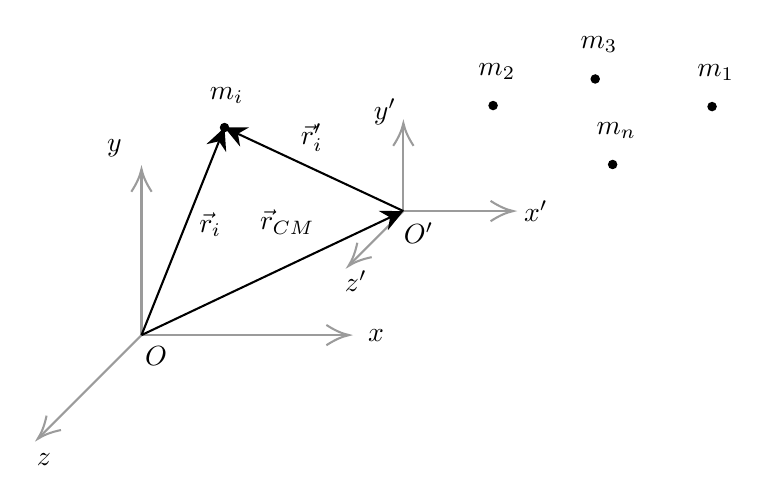
\begin{tikzpicture}[x=0.75pt,y=0.75pt,yscale=-1,xscale=1]
	%uncomment if require: \path (0,300); %set diagram left start at 0, and has height of 300

	%Straight Lines [id:da3973464237777369] 
	\draw [color={rgb, 255:red, 155; green, 155; blue, 155 }  ,draw opacity=1 ]   (190,220) -- (288,220) ;
	\draw [shift={(290,220)}, rotate = 180] [color={rgb, 255:red, 155; green, 155; blue, 155 }  ,draw opacity=1 ][line width=0.75]    (10.93,-4.9) .. controls (6.95,-2.3) and (3.31,-0.67) .. (0,0) .. controls (3.31,0.67) and (6.95,2.3) .. (10.93,4.9)   ;
	%Straight Lines [id:da7302780746120818] 
	\draw [color={rgb, 255:red, 155; green, 155; blue, 155 }  ,draw opacity=1 ]   (190,220) -- (190,142) ;
	\draw [shift={(190,140)}, rotate = 450] [color={rgb, 255:red, 155; green, 155; blue, 155 }  ,draw opacity=1 ][line width=0.75]    (10.93,-4.9) .. controls (6.95,-2.3) and (3.31,-0.67) .. (0,0) .. controls (3.31,0.67) and (6.95,2.3) .. (10.93,4.9)   ;
	%Straight Lines [id:da7635809314408244] 
	\draw [color={rgb, 255:red, 155; green, 155; blue, 155 }  ,draw opacity=1 ]   (190,220) -- (141.41,268.59) ;
	\draw [shift={(140,270)}, rotate = 315] [color={rgb, 255:red, 155; green, 155; blue, 155 }  ,draw opacity=1 ][line width=0.75]    (10.93,-4.9) .. controls (6.95,-2.3) and (3.31,-0.67) .. (0,0) .. controls (3.31,0.67) and (6.95,2.3) .. (10.93,4.9)   ;
	%Straight Lines [id:da9778907913109491] 
	\draw [color={rgb, 255:red, 155; green, 155; blue, 155 }  ,draw opacity=1 ]   (316.18,160.24) -- (367.12,160.24) ;
	\draw [shift={(369.12,160.24)}, rotate = 180] [color={rgb, 255:red, 155; green, 155; blue, 155 }  ,draw opacity=1 ][line width=0.75]    (10.93,-4.9) .. controls (6.95,-2.3) and (3.31,-0.67) .. (0,0) .. controls (3.31,0.67) and (6.95,2.3) .. (10.93,4.9)   ;
	%Straight Lines [id:da5224303885204684] 
	\draw [color={rgb, 255:red, 155; green, 155; blue, 155 }  ,draw opacity=1 ]   (316.18,160.24) -- (316.18,119.88) ;
	\draw [shift={(316.18,117.88)}, rotate = 450] [color={rgb, 255:red, 155; green, 155; blue, 155 }  ,draw opacity=1 ][line width=0.75]    (10.93,-4.9) .. controls (6.95,-2.3) and (3.31,-0.67) .. (0,0) .. controls (3.31,0.67) and (6.95,2.3) .. (10.93,4.9)   ;
	%Straight Lines [id:da8855900305148521] 
	\draw [color={rgb, 255:red, 155; green, 155; blue, 155 }  ,draw opacity=1 ]   (316.18,160.24) -- (291.12,185.29) ;
	\draw [shift={(289.71,186.71)}, rotate = 315] [color={rgb, 255:red, 155; green, 155; blue, 155 }  ,draw opacity=1 ][line width=0.75]    (10.93,-4.9) .. controls (6.95,-2.3) and (3.31,-0.67) .. (0,0) .. controls (3.31,0.67) and (6.95,2.3) .. (10.93,4.9)   ;
	%Straight Lines [id:da05727546365654601] 
	\draw    (190,220) -- (313.47,161.52) ;
	\draw [shift={(316.18,160.24)}, rotate = 514.65] [fill={rgb, 255:red, 0; green, 0; blue, 0 }  ][line width=0.08]  [draw opacity=0] (10.72,-5.15) -- (0,0) -- (10.72,5.15) -- (7.12,0) -- cycle    ;
	%Straight Lines [id:da8494068632959506] 
	\draw    (190,220) -- (228.89,122.79) ;
	\draw [shift={(230,120)}, rotate = 471.8] [fill={rgb, 255:red, 0; green, 0; blue, 0 }  ][line width=0.08]  [draw opacity=0] (10.72,-5.15) -- (0,0) -- (10.72,5.15) -- (7.12,0) -- cycle    ;
	%Straight Lines [id:da8664667653130169] 
	\draw    (316.18,160.24) -- (232.72,121.27) ;
	\draw [shift={(230,120)}, rotate = 385.03] [fill={rgb, 255:red, 0; green, 0; blue, 0 }  ][line width=0.08]  [draw opacity=0] (10.72,-5.15) -- (0,0) -- (10.72,5.15) -- (7.12,0) -- cycle    ;
	%Shape: Circle [id:dp14778114923410857] 
	\draw  [fill={rgb, 255:red, 0; green, 0; blue, 0 }  ,fill opacity=1 ] (228.25,120) .. controls (228.25,119.03) and (229.03,118.25) .. (230,118.25) .. controls (230.97,118.25) and (231.75,119.03) .. (231.75,120) .. controls (231.75,120.97) and (230.97,121.75) .. (230,121.75) .. controls (229.03,121.75) and (228.25,120.97) .. (228.25,120) -- cycle ;
	%Shape: Circle [id:dp1926347954809542] 
	\draw  [fill={rgb, 255:red, 0; green, 0; blue, 0 }  ,fill opacity=1 ] (357.65,109.4) .. controls (357.65,108.43) and (358.43,107.65) .. (359.4,107.65) .. controls (360.37,107.65) and (361.15,108.43) .. (361.15,109.4) .. controls (361.15,110.37) and (360.37,111.15) .. (359.4,111.15) .. controls (358.43,111.15) and (357.65,110.37) .. (357.65,109.4) -- cycle ;
	%Shape: Circle [id:dp9267696113178119] 
	\draw  [fill={rgb, 255:red, 0; green, 0; blue, 0 }  ,fill opacity=1 ] (406.85,96.6) .. controls (406.85,95.63) and (407.63,94.85) .. (408.6,94.85) .. controls (409.57,94.85) and (410.35,95.63) .. (410.35,96.6) .. controls (410.35,97.57) and (409.57,98.35) .. (408.6,98.35) .. controls (407.63,98.35) and (406.85,97.57) .. (406.85,96.6) -- cycle ;
	%Shape: Circle [id:dp21813701641800876] 
	\draw  [fill={rgb, 255:red, 0; green, 0; blue, 0 }  ,fill opacity=1 ] (415.25,137.8) .. controls (415.25,136.83) and (416.03,136.05) .. (417,136.05) .. controls (417.97,136.05) and (418.75,136.83) .. (418.75,137.8) .. controls (418.75,138.77) and (417.97,139.55) .. (417,139.55) .. controls (416.03,139.55) and (415.25,138.77) .. (415.25,137.8) -- cycle ;
	%Shape: Circle [id:dp6494232798227508] 
	\draw  [fill={rgb, 255:red, 0; green, 0; blue, 0 }  ,fill opacity=1 ] (463.15,109.9) .. controls (463.15,108.93) and (463.93,108.15) .. (464.9,108.15) .. controls (465.87,108.15) and (466.65,108.93) .. (466.65,109.9) .. controls (466.65,110.87) and (465.87,111.65) .. (464.9,111.65) .. controls (463.93,111.65) and (463.15,110.87) .. (463.15,109.9) -- cycle ;

	% Text Node
	\draw (303,220) node    {$x$};
	% Text Node
	\draw (177,130) node    {$y$};
	% Text Node
	\draw (143,280) node    {$z$};
	% Text Node
	\draw (380,160.24) node    {$x'$};
	% Text Node
	\draw (307.29,112.59) node    {$y'$};
	% Text Node
	\draw (293.29,194) node    {$z'$};
	% Text Node
	\draw (197,230) node    {$O$};
	% Text Node
	\draw (323.5,171) node    {$O'$};
	% Text Node
	\draw (231,104.67) node    {$m_{i}$};
	% Text Node
	\draw (361.2,93) node    {$m_{2}$};
	% Text Node
	\draw (410.4,80.2) node    {$m_{3}$};
	% Text Node
	\draw (418.8,121.4) node    {$m_{n}$};
	% Text Node
	\draw (223.1,166.9) node    {$\vec{r}_{i}$};
	% Text Node
	\draw (272,125) node    {$\vec{r} '_{i}$};
	% Text Node
	\draw (260.2,165.6) node    {$\vec{r}_{CM}$};
	% Text Node
	\draw (466.7,93.5) node    {$m_{1}$};

	\end{tikzpicture}
\end{figure}
\FloatBarrier
Il generico punto di massa $m_i$ sarà descritto dal vettore posizione $\vec{r}_i$. Si potrà osservare il moto del sistema di punti guardando ciò che accade da un osservatore posto in $O$ oppure sul centro di massa. Quest'ultimo sistema di riferimento prende il nome di \emph{sistema di riferimento del centro di massa}. In genere gli assi vengono presi paralleli e equiversi rispetto a quelli del sistema di riferimento assoluto in $O$.

Si definisce la posizione della generica massa $m_i$ rispetto al sistema di riferimento del centro di massa con il vettore posizione $\vec{r\,'}_i$. Sussiste allora la seguente relazione:

\[
	\forall i: \vec{r}_i = \vec{r}_\text{CM} + \vec{r\,'}_i
\]

Questo discorso si può tradurre anche in termini di velocità. Infatti, per la legge di composizione delle velocità:

\begin{gather*}
	\vec{v}_{\text{ass} } = \vec{v}_{\text{rel} } + \vec{v}_{\text{traslazione}}\\
	\vec{v}_i = \vec{v'}_i + \vec{v}_\text{CM}
\end{gather*}

Si comincia andando a considerare la definizione di momento angolare totale del sistema di punti rispetto al polo $O$ fermo nello spazio.

\begin{figure}[htpb]
	\centering

	\tikzset{every picture/.style={line width=0.75pt}} %set default line width to 0.75pt        

	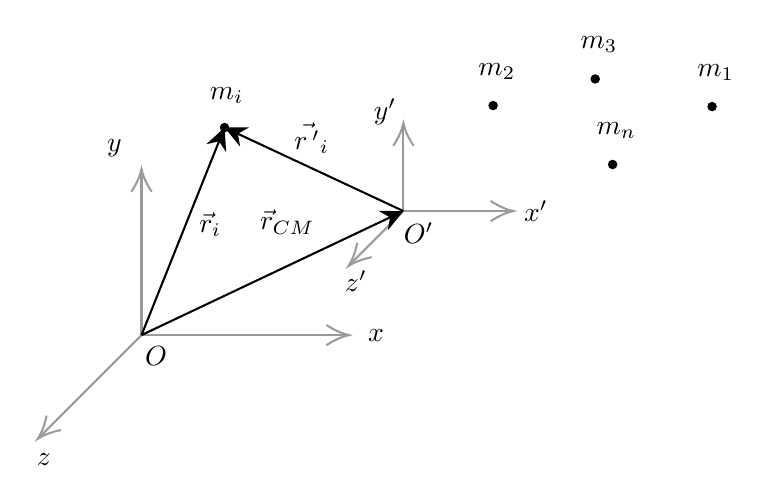
\begin{tikzpicture}[x=0.75pt,y=0.75pt,yscale=-1,xscale=1]
	%uncomment if require: \path (0,300); %set diagram left start at 0, and has height of 300

	%Straight Lines [id:da3973464237777369] 
	\draw [color={rgb, 255:red, 155; green, 155; blue, 155 }  ,draw opacity=1 ]   (190,220) -- (288,220) ;
	\draw [shift={(290,220)}, rotate = 180] [color={rgb, 255:red, 155; green, 155; blue, 155 }  ,draw opacity=1 ][line width=0.75]    (10.93,-4.9) .. controls (6.95,-2.3) and (3.31,-0.67) .. (0,0) .. controls (3.31,0.67) and (6.95,2.3) .. (10.93,4.9)   ;
	%Straight Lines [id:da7302780746120818] 
	\draw [color={rgb, 255:red, 155; green, 155; blue, 155 }  ,draw opacity=1 ]   (190,220) -- (190,142) ;
	\draw [shift={(190,140)}, rotate = 450] [color={rgb, 255:red, 155; green, 155; blue, 155 }  ,draw opacity=1 ][line width=0.75]    (10.93,-4.9) .. controls (6.95,-2.3) and (3.31,-0.67) .. (0,0) .. controls (3.31,0.67) and (6.95,2.3) .. (10.93,4.9)   ;
	%Straight Lines [id:da7635809314408244] 
	\draw [color={rgb, 255:red, 155; green, 155; blue, 155 }  ,draw opacity=1 ]   (190,220) -- (141.41,268.59) ;
	\draw [shift={(140,270)}, rotate = 315] [color={rgb, 255:red, 155; green, 155; blue, 155 }  ,draw opacity=1 ][line width=0.75]    (10.93,-4.9) .. controls (6.95,-2.3) and (3.31,-0.67) .. (0,0) .. controls (3.31,0.67) and (6.95,2.3) .. (10.93,4.9)   ;
	%Straight Lines [id:da9778907913109491] 
	\draw [color={rgb, 255:red, 155; green, 155; blue, 155 }  ,draw opacity=1 ]   (316.18,160.24) -- (367.12,160.24) ;
	\draw [shift={(369.12,160.24)}, rotate = 180] [color={rgb, 255:red, 155; green, 155; blue, 155 }  ,draw opacity=1 ][line width=0.75]    (10.93,-4.9) .. controls (6.95,-2.3) and (3.31,-0.67) .. (0,0) .. controls (3.31,0.67) and (6.95,2.3) .. (10.93,4.9)   ;
	%Straight Lines [id:da5224303885204684] 
	\draw [color={rgb, 255:red, 155; green, 155; blue, 155 }  ,draw opacity=1 ]   (316.18,160.24) -- (316.18,119.88) ;
	\draw [shift={(316.18,117.88)}, rotate = 450] [color={rgb, 255:red, 155; green, 155; blue, 155 }  ,draw opacity=1 ][line width=0.75]    (10.93,-4.9) .. controls (6.95,-2.3) and (3.31,-0.67) .. (0,0) .. controls (3.31,0.67) and (6.95,2.3) .. (10.93,4.9)   ;
	%Straight Lines [id:da8855900305148521] 
	\draw [color={rgb, 255:red, 155; green, 155; blue, 155 }  ,draw opacity=1 ]   (316.18,160.24) -- (291.12,185.29) ;
	\draw [shift={(289.71,186.71)}, rotate = 315] [color={rgb, 255:red, 155; green, 155; blue, 155 }  ,draw opacity=1 ][line width=0.75]    (10.93,-4.9) .. controls (6.95,-2.3) and (3.31,-0.67) .. (0,0) .. controls (3.31,0.67) and (6.95,2.3) .. (10.93,4.9)   ;
	%Straight Lines [id:da05727546365654601] 
	\draw    (190,220) -- (313.47,161.52) ;
	\draw [shift={(316.18,160.24)}, rotate = 514.65] [fill={rgb, 255:red, 0; green, 0; blue, 0 }  ][line width=0.08]  [draw opacity=0] (10.72,-5.15) -- (0,0) -- (10.72,5.15) -- (7.12,0) -- cycle    ;
	%Straight Lines [id:da8494068632959506] 
	\draw    (190,220) -- (228.89,122.79) ;
	\draw [shift={(230,120)}, rotate = 471.8] [fill={rgb, 255:red, 0; green, 0; blue, 0 }  ][line width=0.08]  [draw opacity=0] (10.72,-5.15) -- (0,0) -- (10.72,5.15) -- (7.12,0) -- cycle    ;
	%Straight Lines [id:da8664667653130169] 
	\draw    (316.18,160.24) -- (232.72,121.27) ;
	\draw [shift={(230,120)}, rotate = 385.03] [fill={rgb, 255:red, 0; green, 0; blue, 0 }  ][line width=0.08]  [draw opacity=0] (10.72,-5.15) -- (0,0) -- (10.72,5.15) -- (7.12,0) -- cycle    ;
	%Shape: Circle [id:dp14778114923410857] 
	\draw  [fill={rgb, 255:red, 0; green, 0; blue, 0 }  ,fill opacity=1 ] (228.25,120) .. controls (228.25,119.03) and (229.03,118.25) .. (230,118.25) .. controls (230.97,118.25) and (231.75,119.03) .. (231.75,120) .. controls (231.75,120.97) and (230.97,121.75) .. (230,121.75) .. controls (229.03,121.75) and (228.25,120.97) .. (228.25,120) -- cycle ;
	%Shape: Circle [id:dp1926347954809542] 
	\draw  [fill={rgb, 255:red, 0; green, 0; blue, 0 }  ,fill opacity=1 ] (357.65,109.4) .. controls (357.65,108.43) and (358.43,107.65) .. (359.4,107.65) .. controls (360.37,107.65) and (361.15,108.43) .. (361.15,109.4) .. controls (361.15,110.37) and (360.37,111.15) .. (359.4,111.15) .. controls (358.43,111.15) and (357.65,110.37) .. (357.65,109.4) -- cycle ;
	%Shape: Circle [id:dp9267696113178119] 
	\draw  [fill={rgb, 255:red, 0; green, 0; blue, 0 }  ,fill opacity=1 ] (406.85,96.6) .. controls (406.85,95.63) and (407.63,94.85) .. (408.6,94.85) .. controls (409.57,94.85) and (410.35,95.63) .. (410.35,96.6) .. controls (410.35,97.57) and (409.57,98.35) .. (408.6,98.35) .. controls (407.63,98.35) and (406.85,97.57) .. (406.85,96.6) -- cycle ;
	%Shape: Circle [id:dp21813701641800876] 
	\draw  [fill={rgb, 255:red, 0; green, 0; blue, 0 }  ,fill opacity=1 ] (415.25,137.8) .. controls (415.25,136.83) and (416.03,136.05) .. (417,136.05) .. controls (417.97,136.05) and (418.75,136.83) .. (418.75,137.8) .. controls (418.75,138.77) and (417.97,139.55) .. (417,139.55) .. controls (416.03,139.55) and (415.25,138.77) .. (415.25,137.8) -- cycle ;
	%Shape: Circle [id:dp6494232798227508] 
	\draw  [fill={rgb, 255:red, 0; green, 0; blue, 0 }  ,fill opacity=1 ] (463.15,109.9) .. controls (463.15,108.93) and (463.93,108.15) .. (464.9,108.15) .. controls (465.87,108.15) and (466.65,108.93) .. (466.65,109.9) .. controls (466.65,110.87) and (465.87,111.65) .. (464.9,111.65) .. controls (463.93,111.65) and (463.15,110.87) .. (463.15,109.9) -- cycle ;

	% Text Node
	\draw (303,220) node    {$x$};
	% Text Node
	\draw (177,130) node    {$y$};
	% Text Node
	\draw (143,280) node    {$z$};
	% Text Node
	\draw (380,160.24) node    {$x'$};
	% Text Node
	\draw (307.29,112.59) node    {$y'$};
	% Text Node
	\draw (293.29,194) node    {$z'$};
	% Text Node
	\draw (197,230) node    {$O$};
	% Text Node
	\draw (323.5,171) node    {$O'$};
	% Text Node
	\draw (231,104.67) node    {$m_{i}$};
	% Text Node
	\draw (361.2,93) node    {$m_{2}$};
	% Text Node
	\draw (410.4,80.2) node    {$m_{3}$};
	% Text Node
	\draw (418.8,121.4) node    {$m_{n}$};
	% Text Node
	\draw (223.1,166.9) node    {$\vec{r}_{i}$};
	% Text Node
	\draw (272,125) node    {$\vec{r\,'}_i$};
	% Text Node
	\draw (260.2,165.6) node    {$\vec{r}_{CM}$};
	% Text Node
	\draw (466.7,93.5) node    {$m_{1}$};

	\end{tikzpicture}
\end{figure}
\FloatBarrier
A partire da questa definizione si va a sostituire usando le relazioni trovate sopra:

\begin{equation*}
	\begin{aligned}
		\vec{L}_{tot}^{(o)} &= \sum_i \vec{r}_i\times m_i\vec{v}_i \\
		&= \sum_i (\vec{r'}_i + \vec{r}_\text{CM}) \times m_i (\vec{v'}_i + \vec{v}_\text{CM}) \\
		&= \sum_i m_i \vec{r'}_i \times \vec{v'}_i + \sum_i m_i \, \vec{r'}_i \times \vec{v}_\text{CM} \\
		&\quad + \sum_i m_i\, \vec{r}_\text{CM}\times \vec{v'}_i + \sum_i m_i \, \vec{r}_\text{CM}\times \vec{v}_\text{CM}
	\end{aligned}
\end{equation*}

\begin{enumerate}
	\item Il primo termine dentro la sommatoria lo si chiama \emph{momento angolare di ogni punto materiale rispetto al centro di massa}. È il momento angolare che si attribuisce ad ogni punto nel sistema di riferimento del centro di massa. La somma di tutti questi termini la si chiama $L_{\text{totale}}'$.
	\item Nel secondo termine si nota che dentro la sommatoria c'è un componente che non dipende dal pedice e che quindi si può portare fuori da essa ($\vec{v}_\text{CM}$). $m_i$ è uno scalare: $(\sum_i m_i\vec{r'}_i)\times \vec{v}_\text{CM}$. Il termine tra parentesi è pari a $\vec{r'}_\text{CM} \, M_\text{tot}$, in cui figura la posizione del centro di massa nel sistema di riferimento del centro di massa. Essendo il punto individuato da $\vec{r}_\text{CM}$ coincidente con l'origine di tale sistema di riferimento, si deduce che la sommatoria vale $0$.
	\item Riguardo al terzo termine, si può notare che il vettore posizione del centro di massa non dipende dal pedice $i$ e può essere quindi portato fuori dalla sommatoria. Rimane un termine che contiene la sommatoria:
	\[
		\sum_i (\vec{v'}_i\,m_i ).\quad \quad \vec{v}_{cm} = \sum_i \frac{m_i\vec{v}_i  }{M_{tot} } \quad \vec{v'}_{cm} = \sum_i \frac{m_i\vec{v'}_i}{M_{tot} } = 0
	\]
	Per motivi analoghi, si deduce che anche questo termine è nullo.
	\item Per quanto concerne l'ultimo termine, si può portare fuori dalla sommatoria tutto tranne la massa $i$-esima. Si ha semplicemente la somma di tante masse, che fa la massa totale del sistema. Il termine che si ottiene è il momento angolare del centro di massa rispetto al polo $O$.
\end{enumerate}

Il risultato che si ottiene è il primo teorema di K\"onig, il quale afferma che il momento angolare totale del sistema si può vedere come la somma dei due contributi rilevati.
Il primo informa sulla rotazione intorno al polo del centro di massa. Accanto a questo è sempre necessario tenere conto anche del moto di rotazione delle varie parti del sistema intorno al centro di massa, rappresentato dal secondo termine. Ecco quindi il doppio contributo che entra in gioco nel momento angolare.

\[
	\vec{L}_{tot}^{(o)} = \vec{r}_{cm}\times M_{tot}\,\vec{v}_{cm} + \sum_i (\vec{r'}\times m_i\,\vec{v'}_i)
\]

In tale dimostrazione era fondamentale capire che le quantità del secondo e terzo termine sono nulle.

\begin{gather*}
	\frac{\sum_i m_i\vec{r}_i   }{M_{tot} } = \vec{r'}_{cm} = 0 \qquad \frac{\sum_i m_i\vec{v}_i }{M_{tot} } = \vec{v'}_{cm} = 0 \\
	\boxed{\vec{L}_{tot}^{(o)}   = \vec{L}_{cm}^{(o)} + \vec{L'}_{tot}}
\end{gather*}

\paragraph{Secondo teorema di K\"onig} È possibile enunciare e dimostrare un secondo teorema relativo all'energia cinetica totale del sistema. Esso afferma che l'energia cinetica totale del sistema si può vedere come di nuovo suddivisa in due contributi: l'energia cinetica del solo centro di massa e l'energia cinetica dell'intero sistema rispetto al centro di massa. Si vede che l'energia cinetica del centro di massa e dell'intero sistema saranno:

\[
	E_{K,cm} = \frac{1}{2} M_{tot}\cdot v_{cm}^2 \qquad E_{K,tot} = \sum_i E_{K,i}
\]

Nel secondo termine, in particolare nell'$i$-esima componente, si trova la velocità relativa al centro di massa. La dimostrazione è del tutto analoga:

\[
	E_{K,tot} = \sum_i \frac{1}{2} m_i\,v_i^2
\]

Si va a riscrivere la velocità $i$-esima nella somma vettoriale della velocità del centro di massa e quella relativa al centro di massa:

\[
\vec{v}_i = \vec{v}_{cm} + \vec{v'}
\]

Si noti che vale la relazione $\vec{v}_i \cdot \vec{v}_i = v_i^2$, molto utile per introdurre in una notazione scalare una relazione vettoriale. Si può quindi affermare che:

\[ |\vec{v}_\text{CM}+\vec{v'}|^2= (\vec{v}_\text{CM}+\vec{v'}) \cdot (\vec{v}_\text{CM}+\vec{v'}) \]

Dovranno nascere quattro contributi:

\begin{equation*}
	\begin{aligned}
		E_{K,tot} &= \sum_i \frac{1}{2} m_i (\vec{v}_{cm}+\vec{v'}  ) \cdot (\vec{v}_{cm}+\vec{v'}  ) \\
		&= \sum_i \frac{1}{2} m_i v_{cm}^2 + \sum_i \frac{1}{2} m_i\,\vec{v}_{cm}\cdot \vec{v'}_i + \sum_i \frac{1}{2} m_i \vec{v'} \cdot \vec{v}_{cm} + \sum_i \frac{1}{2} m_i v'^2_i
	\end{aligned}
\end{equation*}

Il secondo e il terzo termine sono del tutto uguali perché il prodotto scalare gode della proprietà commutativa. $\vec{v}_{cm}$ è un termine che non ha un pedice $i$ e che quindi può essere portato fuori dalla sommatoria. Allora si otterrà:

\[
	\vec{v}_{cm} \cdot \sum_i \vec{v'}_i m_i = \vec{v}_{cm}\cdot M_{tot}\cdot \vec{v'}_{cm} = 0
\]
$\vec{v'}_{cm}$ è zero nel sistema di riferimento del centro di massa.
Rimangono soltanto i primo e il quarto termine, che hanno un significato molto semplice da vedere. Il primo termine sarà:

\[
	\frac{1}{2} v_{cm}^2 \sum_i m_i = \frac{1}{2} v_{cm}^2 M_{tot}
\]

Questo termine è l'energia cinetica di un punto che si muove come il centro di massa e che quindi rappresenta l'\textbf{energia cinetica del centro di massa}.
L'ultimo termine rimasto è la somma di tante energie cinetiche dove compare per ogni massa la velocità che essa ha nel sistema di riferimento del centro di massa. Si tratta dell'energia cinetica totale del sistema nel sistema di riferimento del centro di massa.

Il secondo teorema di K\"onig è quindi dato da.

\[
	\boxed{E_{K,tot} = E_{K,cm} + E'_K}
\]

Grazie a questo teorema, si deduce la necessità di tenere conto del fatto che le varie parti del sistema si muovono rispetto al centro di massa e hanno bisogno di una certa energia per mettersi in movimento.
Come per il primo si può affermare che l'energia cinetica non può essere descritta solo in termini del centro di massa.
Questi due teoremi hanno importanza notevole nello studio della dinamica del corpo rigido.
